%pdflatex latexusage
%asy latexusage-*.asy
%pdflatex latexusage


\documentclass{amsart} % A4 paper and 11pt font size
%\usepackage[activate={true,nocompatibility},final,tracking=true,kerning=true,spacing=true,factor=1100,stretch=10,shrink=10]{microtype}

\usepackage{fontspec}
%\setmainfont{Caveat}
%\setmainfont{Kalam Light} 
%\setmainfont{Indie Flower}

%\setmainfont{Indie Flower}[AutoFakeBold=5.0,]%, AutoFakeSlant=0.3]
%\usepackage[T1]{fontenc} % Use 8-bit encoding that has 256 glyphs
%\usepackage{mathpazo} % Use the Adobe Utopia font for the document - comment this line to return to the LaTeX default
\usepackage[english]{babel} % English language/hyphenation
\usepackage{amsmath,amsfonts,amsthm,amssymb} % Math packages
\usepackage{tcolorbox,colortbl}
\tcbuselibrary{theorems}
\usepackage{etoolbox} % Allows customization of theorems
\usepackage{pgf,tikz}
\usetikzlibrary{positioning,matrix,arrows}
\usepackage{float}
\usepackage{tikz-cd}
\usepackage{caption}
\usepackage{stmaryrd}
\usepackage{multicol}
\usepackage{booktabs}
\usepackage{verbatim}
\usepackage{enumerate}
\usepackage{geometry}
\usepackage{python highlight}
\usepackage{fancyhdr} % Custom headers and footers
\usepackage{tikz}
\usepackage{tikz-3dplot}
\usepackage{ifthen}
%\usepackage[active,tightpage]{preview}
\usetikzlibrary{angles,quotes,bending}
\usetikzlibrary{matrix}
\usepackage{hyperref}
\usepackage{tikz}
\usepackage{multicol}
\usepackage{parcolumns}
\usepackage{physics}
\usepackage[inline]{asymptote}
\usepackage[b]{esvect}
\usepackage{arydshln} % for dashed/dotted lines in arrays
% adjust dash length and gap (optional)
\usepackage{enumitem}
\setlength\dashlinedash{2pt}   % length of dash
\setlength\dashlinegap{2pt}    % space between dashes
\setlength\arrayrulewidth{0.3pt} % thickness of the rule


\tikzset{
  >={Latex},
  vec/.style   ={very thick, -{Latex[length=3mm]}},
  ghost/.style ={thick, dashed},
}

\definecolor{panel}{RGB}{198,214,235}


% Customize the appearance of links (optional)
\hypersetup{
    colorlinks=true,    % Colored links instead of boxes
    linkcolor=blue!60!black,     % Color of internal links
    filecolor=blue,  % Color of file links
    urlcolor=cyan,      % Color of external urls
    citecolor=green     % Color of citations
}
%\pagestyle{fancyplain} % Makes all pages in the document conform to the custom headers and footers
\fancyhead{} % No page header - if you want one, create it in the same way as the footers below
\fancyfoot[L]{} % Empty left footer
\fancyfoot[C]{} % Empty center footer
\fancyfoot[R]{\thepage} % Page numbering for right footer
\renewcommand{\headrulewidth}{0pt} % Remove header underlines
\renewcommand{\footrulewidth}{0pt} % Remove footer underlines
\setlength{\headheight}{13.6pt} % Customize the height of the header
\allowdisplaybreaks

%===================================================
% 1) NEW COLOR SCHEME
%===================================================
\definecolor{bigideaColor}{RGB}{4, 102, 1}
\definecolor{bigideaBack}{RGB}{11, 252, 3}
%\colorlet{bigideaColor}{red!90!black}       % BIG IDEA (Deep Red)
%\colorlet{bigideaBack}{red!15!white}        % Bright Red Background

\definecolor{WarnColor}{RGB}{255, 1, 1}
\definecolor{WarnBack}{RGB}{255, 159, 156}
%\colorlet{WarnColor}{orange!85!black}    % Warning (Dark Orange)
%\colorlet{WarnBack}{orange!15!white}     % Bright Orange Background

\colorlet{ThmColor}{blue!80!black}       % Theorem (Royal Blue)
\colorlet{ThmBack}{blue!10!white}        % Light Blue Background

\colorlet{CorColor}{green!70!black}      % Corollary (Deep Green)
\colorlet{CorBack}{green!05!white}       % Light Green Background

\colorlet{PropColor}{blue!75!black}    % Proposition (Dark Purple)
\colorlet{PropBack}{blue!05!white}     % Muted Purple Background

\colorlet{TechColor}{cyan!80!black}      % Technics (Deep Cyan)
\colorlet{TechBack}{cyan!10!white}       % Very Light Cyan Background

\colorlet{DefnColor}{gray!80!black}      % Definition (Dark Gray)
\colorlet{DefnBack}{gray!10!white}       % Very Light Gray Background

%===================================================
% 2) THEOREM STYLES (COLORING THE HEADING TEXT)
%===================================================
\newtheoremstyle{RedThmStyle}   % BIG IDEA (RED)
  {\topsep}{\topsep}
  {\itshape}{0pt}
  {\bfseries\color{bigideaColor}}
  {}{.5em}
  {%
    \noindent
    \thmname{#1}\thmnumber{ #2}\thmnote{ -- \color{bigideaColor}{#3}}
  }

\newtheoremstyle{OrangeThmStyle}   % Warning (ORANGE)
  {\topsep}{\topsep}
  {\itshape}{0pt}
  {\bfseries\color{WarnColor}}
  {}{.5em}
  {%
    \noindent
    \thmname{#1}\thmnumber{ #2}\thmnote{ -- \color{WarnColor}{#3}}
  }

\newtheoremstyle{BlueThmStyle}   % Theorem (BLUE)
  {\topsep}{\topsep}
  {\itshape}{0pt}
  {\bfseries\color{ThmColor}}
  {}{.5em}
  {%
    \noindent
    \thmname{#1}\thmnumber{ #2}\thmnote{ -- \color{ThmColor}{#3}}
  }

\newtheoremstyle{GreenThmStyle}   % Corollary (GREEN)
  {\topsep}{\topsep}
  {\itshape}{0pt}
  {\bfseries\color{CorColor}}
  {}{.5em}
  {%
    \noindent
    \thmname{#1}\thmnumber{ #2}\thmnote{ -- \color{CorColor}{#3}}
  }

\newtheoremstyle{PurpleThmStyle}   % Proposition (PURPLE)
  {\topsep}{\topsep}
  {\itshape}{0pt}
  {\bfseries\color{PropColor}}
  {}{.5em}
  {%
    \noindent
    \thmname{#1}\thmnumber{ #2}\thmnote{ -- \color{PropColor}{#3}}
  }

\newtheoremstyle{CyanThmStyle}   % Technics (CYAN)
  {\topsep}{\topsep}
  {\itshape}{0pt}
  {\bfseries\color{TechColor}}
  {}{.5em}
  {%
    \noindent
    \thmname{#1}\thmnumber{ #2}\thmnote{ -- \color{TechColor}{#3}}
  }

\newtheoremstyle{GrayThmStyle}   % Definition (GRAY)
  {\topsep}{\topsep}
  {\normalfont}{0pt}
  {\bfseries\color{DefnColor}}
  {}{.5em}
  {%
    \noindent
    \thmname{#1}\thmnumber{ #2}\thmnote{ -- \color{DefnColor}{#3}}
  }

%===================================================
% 3) LINK THE STYLES TO ENVIRONMENTS
%===================================================
\theoremstyle{BlueThmStyle}
\newtheorem{thm}{Theorem} % Define first

\theoremstyle{RedThmStyle}
\newtheorem{bigidea}[thm]{BIG IDEA} % Now it works

\theoremstyle{OrangeThmStyle}
\newtheorem{warn}[thm]{Warning} % Now it works

\theoremstyle{GreenThmStyle}
\newtheorem{cor}[thm]{Corollary}

\theoremstyle{PurpleThmStyle}
\newtheorem{prop}[thm]{Proposition}

\theoremstyle{CyanThmStyle}
\newtheorem{tech}[thm]{Technics}

\theoremstyle{GrayThmStyle}
\newtheorem{defn}[thm]{Definition}

\theoremstyle{GrayThmStyle}
\newtheorem{notns}[thm]{Notations}

%===================================================
% 4) TCOLORBOXENVIRONMENTS (BOX COLORS)
%===================================================
\tcolorboxenvironment{bigidea}{
  colback=bigideaBack,
  colframe=bigideaColor
}

\tcolorboxenvironment{warn}{
  colback=WarnBack,
  colframe=WarnColor
}

\tcolorboxenvironment{thm}{
  colback=ThmBack,
  colframe=ThmColor
}

\tcolorboxenvironment{cor}{
  colback=CorBack,
  colframe=CorColor
}

\tcolorboxenvironment{prop}{
  colback=PropBack,
  colframe=PropColor
}

\tcolorboxenvironment{tech}{
  colback=TechBack,
  colframe=TechColor
}

\tcolorboxenvironment{defn}{
  colback=DefnBack,
  colframe=DefnColor
}

\tcolorboxenvironment{notns}{
  colback=DefnBack,
  colframe=DefnColor
}


\everymath{\displaystyle}
\parindent =0pt


%\geometry{
%	left=13mm, % left margin
%	textwidth=130mm, % main text block
%	marginparsep=8mm, % gutter between main text block and margin notes
%	marginparwidth=55mm % width of margin notes
%}
\fontsize{10}{20}\selectfont
%----------------------------------------------------------------------------------------
%	TITLE SECTION
%----------------------------------------------------------------------------------------

\geometry{
    letterpaper,
    width=170mm,
    height=237mm,
%    left=15mm,
 %   top=20mm,
}

\title{	
	%\normalfont\normalsize 
	%{Harvard University - Fall 2024} \\ [0pt] % Your university, school and/or department name(s)
	{\small Summary Notes  -- Harvard Math 21b, Linear Algebra \& Differential Equations }% The assignment title
}\author{} % Your name
\date{\vspace{-5pt}\normalsize \today} % Today's date or a custom date
%\date{}
\begin{document}
\maketitle
%\setcounter{tocdepth}{1}

\tableofcontents

\section{Linear Equations}
\
\\
\subsection{Introduction to Linear Systems}
\
\\

\begin{defn}[Linear Combination]
\
\\
A \textbf{linear combination} of $x_1, \ldots, x_n$ has the form
\begin{equation*}
   a_1x_1+a_2x_2+a_3x_3+\cdots+a_nx_n
\end{equation*}
where the numbers $a_1, \ldots,a_n\in \mathbb{R}$ are the combination's \textbf{coefficients}\footnote{Sometimes we replace $\mathbb{R}$ with another field like $\mathbb{Q}$ or $\mathbb{C}$.}.
\end{defn}

\begin{defn}[Linear Equation]\label{def-sys}
\
\\
A \textbf{linear equation} in the variables $x_1, \ldots, x_n$ has the form
$a_1x_1+a_2x_2+a_3x_3+\cdots+a_nx_n=d$
where $d\in \mathbb{R}$ is the \textbf{constant}.

An $n$-tuple $(s_1,s_2,\ldots,s_n)\in \mathbb{R}^n$ is a \textbf{solution} of, or \textbf{satisfies}, that equation if substituting the numbers $s_1, \ldots, s_n$ for the variables gives a true statement: $a_1s_1+a_2s_2+\cdots+a_ns_n=d$.

A \textbf{system of linear equations}
\[
\begin{aligned}
a_{1,1} x_1+a_{1,2} x_2+\cdots+a_{1, n} x_n & =d_1 \\
a_{2,1} x_1+a_{2,2} x_2+\cdots+a_{2, n} x_n & =d_2 \\
& \vdots \\
a_{m, 1} x_1+a_{m, 2} x_2+\cdots+a_{m, n} x_n & =d_m
\end{aligned}
\]
has the solution $(s_1,s_2,\ldots,s_n)$ if that $n$-tuple is a solution of all of the equations.
\end{defn}


\begin{defn}[Number of solutions of a linear system]
\
\\
A system of equations is said to be \textbf{consistent} if there is at least one solution; it is \textbf{inconsistent} if there are no solutions.
\end{defn}



\begin{thm}[Gauss's Method a.k.a Gauss-Jordan or Row Reduction] \label{th:GaussMethod}
\
\\
If a linear system is changed to another by one of these operations
\begin{enumerate}
  \item an equation is swapped with another
  \item an equation has both sides multiplied by a nonzero constant
  \item an equation is replaced by the sum of itself and a multiple of another
\end{enumerate}
then the two systems have the same set of solutions.
\end{thm}


\begin{defn}[Reduced row-echelon form]
\
\\
A matrix is said to be in \textbf{reduced row-echelon form (rref)} if it satisfies all of the following conditions
\begin{enumerate}
  \item 
If a row has nonzero entries, then the first nonzero entry is a 1, called \textbf{the leading 1 (or pivot)} in this row.
  \item 
If a column contains a leading 1, then all the other entries in that column are 0 .
  \item   
If a row contains a leading 1, then each row above it contains a leading 1 further to the left.
\end{enumerate}
The last condition implies that rows of 0's, if any, appear at the bottom of the matrix.

\end{defn}

\begin{defn}[Elementary Reduction Operations] \label{df:GaussMethod}
\
\\
The three operations from Theorem \ref{th:GaussMethod} are the \textbf{elementary reduction operations}, or \textbf{row operations}, or \textbf{Gaussian operations}. They are:
\begin{itemize}
\item \textbf{swapping}
\item \textbf{multiplying by a scalar} (or \textbf{rescaling})
\item \textbf{row combination}
\end{itemize}
\end{defn}

\begin{defn}[Echelon Form]
\
\\
A system is in \textbf{echelon form} if each leading variable (first nonzero variable in each equation) is to the right of the leading variable in the row above it, with any all-zero rows at the bottom.
\end{defn}

\begin{defn}[Free Variables] \label{df:FreeVars}
\
\\
In an echelon form linear system the variables that are not leading are \textbf{free}.
\end{defn}

\begin{cor}[Solution Set Types]
\
\\
Solution sets of linear systems are either 
\begin{itemize}
\item 
empty, 
\item
have one element, or 
\item
have infinitely many elements.
\end{itemize}
\end{cor}


\begin{thm}[Inconsistent Systems]
\
\\
A linear system is inconsistent if (and only if) the reduced row-echelon form of its augmented matrix contains the row $\left[\begin{array}{llll:l}0 & 0 & \cdots & 0 & 1\end{array}\right]$, representing the equation $0=1$.

If a linear system is consistent, then it has either

- infinitely many solutions (if there is at least one free variable), or

- exactly one solution (if all the variables are leading).

\end{thm}
\begin{thm}[General Solution Form]
\
\\
Any linear system's solution set has the form $\{p + c_1\beta_1 + \cdots + c_k\beta_k \mid c_1,\ldots,c_k \in \mathbb{R}\}$ where $p$ is any particular solution and $k$ equals the number of free variables.
\end{thm}

\begin{defn}[Matrix]
\
\\
An $m \times n$ \textbf{matrix} is a rectangular array of numbers with $m$ rows and $n$ columns. Each number is an \textbf{entry}.
\end{defn}

\begin{defn}[Vector]
\
\\
A \textbf{column vector} is a matrix with a single column. A \textbf{row vector} has a single row. Entries are called \textbf{components}.
\end{defn}

\begin{defn}[Vector Sum]
\
\\
The \textbf{vector sum} of $\vv{u}$ and $\vv{v}$ is the vector of the sums (component-wise addition).
\end{defn}

\begin{defn}[Scalar Multiplication]
\
\\
The \textbf{scalar multiplication} of real number $r$ and vector $\vv{v}$ is the vector of the multiples.
\end{defn}

\begin{defn}[Homogeneous Equation]
\
\\
A \textbf{homogeneous equation} is a linear equation with constant of zero: $a_1x_1+\cdots+a_nx_n=0$.
\end{defn}

\begin{defn}[Nonsingular Matrix]
\
\\
A square matrix is \textbf{nonsingular} if it is the matrix of coefficients of a homogeneous system with a unique solution. Otherwise it is \textbf{singular}.
\end{defn}



\begin{defn}[Linear System]
\
\\
A \textbf{linear system} in variables $x_1,\dots,x_n$ is a collection of equations
$a_{i1}x_1+\cdots+a_{in}x_n=b_i$. Its solution set is an affine subspace of $\mathbb{R}^n$ (possibly empty).
\end{defn}

\begin{defn}[Matrix Form $Ax=b$]
\
\\
The \textbf{coefficient matrix} $A\in\mathbb{R}^{m\times n}$, \textbf{unknown vector} $x\in\mathbb{R}^n$, and \textbf{right-hand side} $b\in\mathbb{R}^m$ define the system $Ax=b$.
\end{defn}

\begin{thm}[Existence and Uniqueness]
\
\\
The system $Ax=b$ has a solution iff $b$ lies in the column space of $A$ (the image). If a solution exists, it is unique iff $\ker(A)=\{0\}$, equivalently $\operatorname{rank}(A)=n$.
\end{thm}

\subsection{Matrices, Vectors, and Gauss--Jordan Elimination}
\
\\

\begin{defn}[Vectors and vector spaces]
\
\\
A matrix with only one column is called a \textbf{column vector}, or simply a \textbf{vector}. The entries of a vector are called its \textbf{components}. The set of all column vectors with $n$ components is denoted by $\mathbb{R}^n$; we will refer to $\mathbb{R}^n$ as a vector space.

A matrix with only one row is called a \textbf{row vector}.
In this text, the term vector refers to column vectors, unless otherwise stated.
\end{defn}

\begin{defn}[Elementary Row Operations]
\
\\
(1) Swap two rows. \\
(2) Multiply a row by a nonzero scalar. \\ 
(3) Replace a row by itself plus a multiple of another row. These preserve the solution set of $Ax=b$.
\end{defn}

\begin{thm}[Reduced Row-Echelon Form (RREF)]
\
\\
Every matrix is row-equivalent to a unique RREF. \textbf{Pivot} columns correspond to \textbf{leading variables}; non-pivot columns correspond to \textbf{free variables} that parametrize the solution set.
\end{thm}

\subsection{On the Solutions of Linear Systems; Matrix Algebra}
\
\\

\begin{thm}[Number of solutions of a linear system]
\
\\
A system of equations is said to be consistent if there is at least one solution; it is inconsistent if there are no solutions.\\
A linear system is inconsistent if (and only if) the reduced row-echelon form of its augmented matrix contains the row $\left[\begin{array}{llll:l}0 & 0 & \cdots & 0 & 1\end{array}\right]$, representing the equation $0=1$.\\
If a linear system is consistent, then it has either\\
- infinitely many solutions (if there is at least one free variable), or\\
- exactly one solution (if all the variables are leading).
\end{thm}

\begin{defn}[Rank of a Matrix (preliminary definition)]
\
\\
The rank of a matrix $A$ is the number of leading 1 's in $\operatorname{rref}(A)$, denoted $\operatorname{rank}(A)$.
\end{defn}

\begin{thm}[Number of equations vs. number of unknowns]
\
\\
If a linear system has exactly one solution, then there must be at least as many equations as there are variables ( $m \leq n$ with the notation from Definition \ref{def-sys}).

Equivalently, we can formulate the contrapositive:\\
A linear system with fewer equations than unknowns $(n<m)$ has either no solutions or infinitely many solutions.
\end{thm}


\begin{thm}[The product $A \vv{x}$ in terms of the columns of $A$]
\
\\
If the column vectors of an $n \times m$ matrix $A$ are $\vv{v}_1, \ldots, \vv{v}_m$ and $\vv{x}$ is a vector in $\mathbb{R}^m$ with components $x_1, \ldots, x_m$, then
\[
A \vv{x}=\left[\begin{array}{ccc}
\mid & & \mid \\
\vv{v}_1 & \ldots & \vv{v}_m \\
\mid & & \mid
\end{array}\right]\left[\begin{array}{c}
x_1 \\
\vdots \\
x_m
\end{array}\right]=x_1 \vv{v}_1+\cdots+x_m \vv{v}_m
\]
\end{thm}



\begin{defn}[Linear combinations]
\
\\
A vector $\vv{b}$ in $\mathbb{R}^n$ is called a linear combination of the vectors $\vv{v}_1, \ldots, \vv{v}_m$ in $\mathbb{R}^n$ if there exist scalars $x_1, \ldots, x_m$ such that
\[
\vv{b}=x_1 \vv{v}_1+\cdots+x_m \vv{v}_m
\]
\end{defn}


\begin{defn}[Matrix Operations]
\
\\
Matrix addition, scalar multiplication, and multiplication $(AB)_{ij}=\sum_k A_{ik}B_{kj}$; the identity $I_n$ satisfies $I_nx=x$.
\end{defn}

\begin{thm}[Rank--Nullity]
\
\\
For $A\in\mathbb{R}^{m\times n}$, $\operatorname{rank}(A)+\dim\ker(A)=n$.
\end{thm}

\section{Linear Transformations}
\
\\
\subsection{Introduction to Linear Transformations and Their Inverses}
\
\\
\begin{defn}[Linear Transformation]
\
\\
A map $T:V\to W$ is \textbf{linear} if $T(u+v)=T(u)+T(v)$ and $T(\alpha v)=\alpha T(v)$. It is invertible (has a linear inverse) iff it is bijective.
\end{defn}

\begin{thm}[Invertibility Criteria on $\mathbb{R}^n$]
\
\\
For $T:\mathbb{R}^n\to\mathbb{R}^n$ with matrix $A$, the following are equivalent: \\(i) $T$ invertible; \\
(ii) $\det A\neq 0$; \\
(iii) $\ker(A)=\{0\}$; \\
(iv) $\Im(A)=\mathbb{R}^n$.
\end{thm}


\begin{thm}[The columns of the matrix of a linear transformation]
\
\\
Consider a linear transformation $T$ from $\mathbb{R}^m$ to $\mathbb{R}^n$. Then, the matrix of $T$ is

\[
A=\left[\begin{array}{cccc}
\mid & \mid & & \mid \\
T\left(\vec{e}_1\right) & T\left(\vec{e}_2\right) & \ldots & T\left(\vec{e}_m\right) \\
\mid & \mid & & \mid
\end{array}\right], \quad \text { where } \quad \vec{e}_i=\left[\begin{array}{c}
0 \\
\vdots \\
0 \\
1 \\
0\\
\vdots \\
0 
\end{array}\right] \leftarrow i \text { th }
\]
\end{thm}
\subsection{Linear Transformations in Geometry}
\
\\
\begin{prop}[Geometric Examples]
\
\\
Rotations, reflections, orthogonal projections, and shears on $\mathbb{R}^2$ or $\mathbb{R}^3$ are linear and each is represented by a matrix in the standard basis.
\end{prop}

\begin{defn}[Orthogonal Projections]
\
\\
Consider a line $L$ in the coordinate plane, running through the origin. Any vector $\vec{x}$ in $\mathbb{R}^2$ can be written uniquely as
\[
\vec{x}=\vec{x}^{\|}+\vec{x}^{\perp},
\]
where $\vec{x}^{\|}$ is parallel to line $L$, and $\vec{x}^{\perp}$ is perpendicular to $L$.
The transformation $T(\vec{x})=\vec{x}^{\|}$ from $\mathbb{R}^2$ to $\mathbb{R}^2$ is called the orthogonal projection of $\vec{x}$ onto $L$, often denoted by $\operatorname{proj}_L(\vec{x})$. If $\vec{w}$ is a nonzero vector parallel to $L$, then
\[
\operatorname{proj}_L(\vec{x})=\left(\frac{\vec{x} \cdot \vec{w}}{\vec{w} \cdot \vec{w}}\right) \vec{w} .
\]
In particular, if $\vec{u}=\begin{bmatrix}u_1 \\ u_2\end{bmatrix}$ is a unit vector parallel to $L$, then
\[
\operatorname{proj}_L(\vec{x})=(\vec{x} \cdot \vec{u}) \vec{u} .
\]
The transformation $T(\vec{x})=\operatorname{proj}_L(\vec{x})$ is linear, with matrix
\[
P=\frac{1}{w_1^2+w_2^2}\begin{bmatrix}
w_1^2 & w_1 w_2 \\
w_1 w_2 & w_2^2
\end{bmatrix}=\begin{bmatrix}
u_1^2 & u_1 u_2 \\
u_1 u_2 & u_2^2
\end{bmatrix} .
\]
\end{defn}

\begin{center}

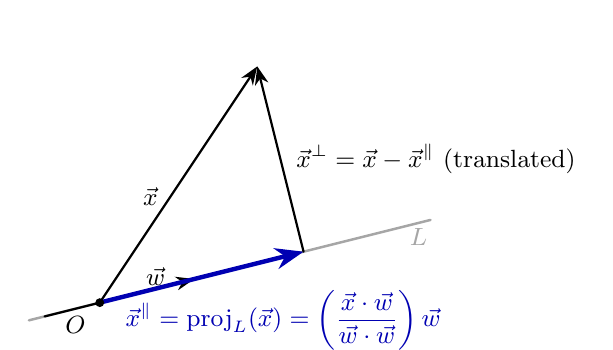
\begin{tikzpicture}[>=Stealth, line cap=round, thick,
  vec/.style={-Stealth},
  axis/.style={line width=0.9pt,gray!70},
  note/.style={font=\small}
]

%--- Geometry setup ---
% Line L direction vector (along \vec{w})
\def\uX{1.0}
\def\uY{0.25}

% Origin and main vector x
\coordinate (O) at (0,0);
\coordinate (x) at (2,3);

% A long copy of L for display
\draw[axis] ($ (O) + -0.9*(\uX,\uY) $) -- ($ (O) + 4.2*(\uX,\uY) $);
\node[note,gray!70, below] at ($ (O) + 3.9*(\uX,\uY) + (0.15,0.1) $) {$L$};

% Vector w (along L)
\draw[vec] ($ (O) - 0.7*(\uX,\uY) $) -- ($ (O) + 1.2*(\uX,\uY) $);
\node[note, above] at ($ (O) + .81*(\uX,\uY) + (-0.1,-0.12) $) {$\vec{w}$};

% Compute a concrete projection point P = proj_L(x) using precomputed numbers
% (for \vec{w}=(1,0.25) and \vec{x}=(2,3)):
%   t = (x·w)/(w·w) = 2.75 / 1.0625 ≈ 2.588235...
%   P = t * w = (2.588, 0.647)
\coordinate (P) at (2.588,0.647);

% Draw x (black) and x_parallel (blue)
\draw[vec] (O) -- (x) node[pos=0.45,left=1pt, note] {$\vec{x}$};
\draw[vec, ultra thick, blue!70!black] (O) -- (P)
  node[pos=0.9, below=8pt, note, blue!70!black]
  {$\vec{x}^{\parallel}=\mathrm{proj}_L(\vec{x})=
  \left(\dfrac{\vec{x}\cdot\vec{w}}{\vec{w}\cdot\vec{w}}\right)\vec{w}$};

% Show the translated perpendicular component from P to x
\draw[vec] (P) -- (x)
  node[midway, right=2pt, note]
  {$\vec{x}^{\perp}=\vec{x}-\vec{x}^{\parallel}$ (translated)};

% Labels for O
\fill (O) circle (1.6pt) node[below left=2pt, note] {$O$};

\end{tikzpicture}

\end{center}

\begin{defn}[Reflections]
\
\\
Consider a line $L$ in the coordinate plane, running through the origin, and let $\vec{x}=\vec{x}^{\|}+\vec{x}^{\perp}$ be a vector in $\mathbb{R}^2$. The linear transformation $T(\vec{x})=\vec{x}^{\|}-\vec{x}^{\perp}$ is called the reflection of $\vec{x}$ about $L$, often denoted by $\operatorname{ref}_L(\vec{x})$ :
\[
\operatorname{ref}_L(\vec{x})=\vec{x}^{\|}-\vec{x}^{\perp}
\]
We have a formula relating $\operatorname{ref}_L(\vec{x})$ to $\operatorname{proj}_L(\vec{x})$ :
\[
\operatorname{ref}_L(\vec{x})=2 \operatorname{proj}_L(\vec{x})-\vec{x}=2(\vec{x} \cdot \vec{u}) \vec{u}-\vec{x} \qquad \text{ where } \vec{u} \text{ is a unit vector on }L.
\]
The matrix of $T$ is of the form $\begin{bmatrix}a & b \\ b & -a\end{bmatrix}$, where $a^2+b^2=1$. Conversely, any matrix of this form represents a reflection about a line.
\end{defn}

\begin{center}
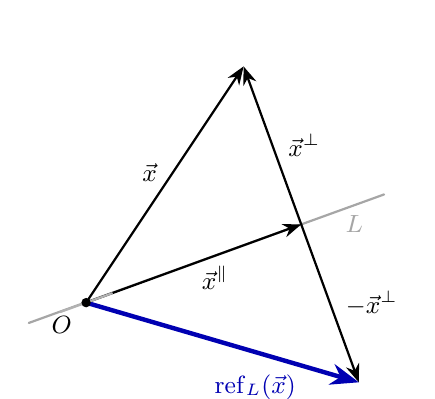
\begin{tikzpicture}[>=Stealth, line cap=round, thick,
  vec/.style={-Stealth},
  grayline/.style={line width=0.8pt,gray!70},
  note/.style={font=\small}
]

%--- Parameters (numerical coordinates for clarity) ---
% Direction of line L (unit-ish): angle ~ 20 degrees
\def\uX{0.94}
\def\uY{0.34}

% Base point through which L passes (slightly above O so L doesn't go through O)
\coordinate (A) at (0.4,0.15);
\coordinate (B) at ($(A)+2.8*(\uX,\uY)$);

% Origin and vector x tip
\coordinate (O) at (0,0);
\coordinate (x) at (2,3);

% Decomposition of x into parallel and perpendicular (precomputed)
% x_parallel = (2.732, 0.994)
% x_perp     = x - x_parallel = (-0.732, 2.006)
\coordinate (xpar) at (2.732,0.994);
\coordinate (xperp) at ($(x)-(xpar)$);

% Two translated copies of x_perp (placed so their midpoints lie on L)
% Choose the projection point on L roughly near (xpar)
\coordinate (P) at (1.9,0.62);  % a point on L used as the "translation anchor"
\coordinate (xperpUp)   at ($(P)+(0.0,1.6)$);
\coordinate (xperpDown) at ($(P)-(0.0,1.6)$);

% Reflection: x_ref = x_parallel - x_perp
\coordinate (xref) at ($(xpar)- (xperp)$);

%--- Draw L ---
\draw[grayline] ($(A)-1.2*(\uX,\uY)$) -- ($(B)+0.8*(\uX,\uY)$);
\node[note,gray!70, below] at ($(B)+0.4*(\uX,\uY)$) {$L$};

%--- Main vectors ---
\draw[vec] (O) -- (x) node[pos=0.55, left=2pt, note] {$\vec{x}$};
\draw[vec] (O) -- (xpar) node[pos=0.6, below, note] {$\vec{x}^{\parallel}$};

% The perpendicular component (shown from tip of x_parallel to x)
\draw[vec] (xpar) -- (x) node[midway, right=2pt, note] {$\vec{x}^{\perp}$};

% Translated copies of +/- x_perp placed with their feet on L
%\draw[vec] (P) -- (xperpUp)
%  node[pos=0.6, right=2pt, note] {$\vec{x}^{\perp}$ (translated)};
%\draw[vec] (P) -- ($(P)-(xperp)$)
%  node[pos=0.55, right=2pt, note] {$-\vec{x}^{\perp}$ (translated)};
\draw[vec] (xpar) -- (xref) 
  node[midway, right=2pt, note] {$-\vec{x}^{\perp}$};
  
% Reflection vector in blue
\draw[vec, ultra thick, blue!70!black] (O) -- (xref)
  node[pos=0.62, below=4pt, note, blue!70!black] {$\mathrm{ref}_L(\vec{x})$};

%--- Origin and small baseline hint for O on an extension of L ---
\draw[gray!60, line width=0.8pt] ($(O)+-0.35*(\uX,\uY)$) -- ($(O)+0.35*(\uX,\uY)$);
\fill (O) circle (1.7pt) node[below left=2pt, note] {$O$};

\end{tikzpicture}
\end{center}


\subsection{Matrix Products}
\
\\
\begin{defn}[Matrix multiplication]
\
\\
a. Let $B$ be an $n \times p$ matrix and $A$ a $q \times m$ matrix. The product $B A$ is defined if (and only if) $p=q$.\\
b. If $B$ is an $n \times p$ matrix and $A$ a $p \times m$ matrix, then the product $B A$ is defined as the matrix of the linear transformation $T(\vv{x})=B(A \vv{x})$. This means that $T(\vv{x})=B(A \vv{x})=(B A) \vv{x}$, for all $\vv{x}$ in the vector space $\mathbb{R}^m$. The product $B A$ is an $n \times m$ matrix.
\end{defn}

\begin{thm}[Composition $\leftrightarrow$ Product]
\
\\
If $S:U\to V$ and $T:V\to W$ have matrices $[S]$ and $[T]$ in chosen bases, then $[T\circ S]=[T][S]$.
\end{thm}

\begin{thm}[The columns of the matrix product]
\
\\
Let $B$ be an $n \times p$ matrix and $A$ a $p \times m$ matrix with columns $\vv{v}_1, \vv{v}_2, \ldots, \vv{v}_m$. Then, the product $B A$ is
\[
B A=B\left[\begin{array}{cccc}
\mid & \mid & & \mid \\
\vv{v}_1 & \vv{v}_2 & \cdots & \vv{v}_m \\
\mid & \mid & & \mid
\end{array}\right]=\left[\begin{array}{cccc}
\mid & \mid & & \mid \\
B \vv{v}_1 & B \vv{v}_2 & \cdots & B \vv{v}_m \\
\mid & \mid & & \mid
\end{array}\right] .
\]
To find $B A$, we can multiply $B$ by the columns of $A$ and combine the resulting vectors.
\end{thm}

\begin{thm}[The entries of the matrix product]
\
\\
Let $B$ be an $n \times p$ matrix and $A$ a $p \times m$ matrix. The $i j$ th entry of $B A$ is the dot product of the $i$ th row of $B$ with the $j$ th column of $A$.
\[
BA =
\begin{bmatrix}
b_{11} & b_{12} & \cdots & b_{1p} \\
b_{21} & b_{22} & \cdots & b_{2p} \\
\vdots & \vdots &        & \vdots \\
\rowcolor{gray!40} b_{i1} & b_{i2} & \cdots & b_{ip} \\
\vdots & \vdots &        & \vdots \\
b_{n1} & b_{n2} & \cdots & b_{np}
\end{bmatrix}
\begin{bmatrix}
a_{11} & a_{12} &\cdots & \cellcolor{gray!40} a_{1j} & \cdots & a_{1m} \\
a_{21} & a_{22} & \cdots & \cellcolor{gray!40} a_{2j} & \cdots & a_{2m} \\
\vdots & \vdots & \vdots & \cellcolor{gray!40} \vdots &        & \vdots \\
a_{p1} & a_{p2} & \cdots & \cellcolor{gray!40} a_{pj} & \cdots & a_{pm}
\end{bmatrix}
\]
is the $n \times m$ matrix whose $i j$ th entry is
\[
b_{i 1} a_{1 j}+b_{i 2} a_{2 j}+\cdots+b_{i p} a_{p j}=\sum_{k=1}^p b_{i k} a_{k j} .
\]
\end{thm}

\begin{prop}[Matrix Properties]
\
\\
\textbf{Multiplying with the identity matrix}

For an $n \times m$ matrix $A$,
\[
A I_m=I_n A=A
\]


\textbf{Matrix multiplication is associative}
\[
(A B) C=A(B C)
\]

\textbf{Distributive property for matrices}

If $A$ and $B$ are $n \times p$ matrices, and $C$ and $D$ are $p \times m$ matrices, then
\[
\begin{aligned}
& A(C+D)=A C+A D, \quad \text { and } \\
& (A+B) C=A C+B C
\end{aligned}
\]

If $A$ is an $n \times p$ matrix, $B$ is a $p \times m$ matrix, and $k$ is a scalar, then
\[
(k A) B=A(k B)=k(A B) .
\]

\end{prop}

\begin{warn}[Not as simple as numbers]
\
\\
If $A,B, C$ are $n\times n$ matrices, in general
\begin{itemize}
\item
$A B \neq B A$ (when they are equal we say that $A$ and $B$ commute)
\item
$(A+B)^2=A^2+A B+B A+B^2 \neq A^2+2A B+B^2$
\item
We could have $A \neq 0, B \neq 0$ but $A B=0$
\item
We could have $A B=0$ and $B A \neq 0$
\item
$AC =AB$ does not imply that $B=C$ (but it does when $A$ is non singular/invertible).
\end{itemize}
\end{warn}


\subsection{The Inverse of a Linear Transformation}
\
\\

\begin{defn}[Invertible matrices]
\
\\
A square matrix $A$ is said to be invertible if the linear transformation $\vv{y}=T(\vv{x})=A \vv{x}$ is invertible. In this case, the matrix of $T^{-1}$ is denoted by $A^{-1}$. If the linear transformation $\vv{y}=T(\vv{x})=A \vv{x}$ is invertible, then its inverse is $\vv{x}=T^{-1}(\vv{y})=A^{-1} \vv{y}$.
\end{defn}





\begin{thm}[Invertibility]
\
\\
An $n \times n$ matrix $A$ is invertible if and only if
\[
\operatorname{rref}(A)=I_n
\]
or, equivalently, if and only if
\[
\operatorname{rank}(A)=n.
\]

\end{thm}

\begin{tech}[Computing $A^{-1}$]
\
\\
If $A$ is invertible, then $A^{-1}$ is obtained by Gauss--Jordan on $\bigl[\,A\,|\,I\,\bigr]$. Moreover, $[T^{-1}]=[T]^{-1}$ for invertible $T$.
\end{tech}

\begin{thm}[Invertibility and linear systems]
\
\\
Let $A$ be an $n \times n$ matrix.
\begin{enumerate}
\item
Consider a vector $\vv{b}$ in $\mathbb{R}^n$. If $A$ is invertible, then the system $A \vv{x}=\vv{b}$ has the unique solution $\vv{x}=A^{-1} \vv{b}$. If $A$ is noninvertible, then the system $A \vv{x}=\vv{b}$ has infinitely many solutions or none.
\item 
Consider the special case when $\vv{b}=\overrightarrow{0}$. The system $A \vv{x}=\overrightarrow{0}$ has $\vv{x}=\overrightarrow{0}$ as a solution. If $A$ is invertible, then this is the only solution. If $A$ is noninvertible, then the system $A \vv{x}=\overrightarrow{0}$ has infinitely many solutions.
\end{enumerate}
\end{thm}


\begin{warn}[The inverse of a product of matrices]
\
\\
If $A$ and $B$ are invertible $n \times n$ matrices, then $B A$ is invertible as well, and
\[
(B A)^{-1}=A^{-1} B^{-1}
\]
Pay attention to the order of the matrices. (Order matters!)
\end{warn}


\begin{thm}[A criterion for invertibility]
\
\\
Let $A$ and $B$ be two $n \times n$ matrices such that
\[
B A=I_n
\]
Then\\
a. $A$ and $B$ are both invertible,\\
b. $A^{-1}=B$ and $B^{-1}=A$, and\\
c. $A B=I_n$.
\end{thm}


\begin{cor}[Inverse of a $2\times 2$ matrix]
\
\\
The $2 \times 2$ matrix
$ A=\begin{bmatrix}
a & b \\
c & d
\end{bmatrix}
$
is invertible if (and only if) $a d-b c \neq 0$.
Quantity $a d-b c$ is called the \textbf{determinant} of $A$, written $\det (A)$
\[
\det (A)=\det \begin{bmatrix}
a & b \\
c & d
\end{bmatrix}=a d-b c .
\]


If $A=\begin{bmatrix}
a & b \\
c & d
\end{bmatrix}
$
is invertible, then
\[
\begin{bmatrix}
a & b \\
c & d
\end{bmatrix}^{-1}=\frac{1}{a d-b c}\begin{bmatrix}
d & -b \\
-c & a
\end{bmatrix}=\frac{1}{\det (A)}\begin{bmatrix}
d & -b \\
-c & a
\end{bmatrix} .
\]
\end{cor}


\begin{thm}[Various characterizations of invertible matrices]
\
\\
For an $n \times n$ matrix $A$, the following statements are equivalent; that is, for a given $A$, they are either all true or all false
\begin{itemize}
\item[i.] $A$ is invertible.
\item[ii.] The linear system $A \vec{x}=\vec{b}$ has a unique solution $\vec{x}$, for all $\vec{b}$ in $\mathbb{R}^n$.
\item[iii.] $\operatorname{rref}(A)=I_n$.
\item[iv.] $\operatorname{rank}(A)=n$.
\item[v.] $\operatorname{im}(A)=\mathbb{R}^n$.
\item[vi.] $\operatorname{ker}(A)=\{\vec{0}\}$.
\item[vii.] $\det A \neq 0$. 
\end{itemize}

\end{thm}


\section{Subspaces of $\mathbb{R}^n$ and Their Dimensions}
\subsection{Image and Kernel of a Linear Transformation}
\
\\

\begin{defn}[Span]
\
\\
Consider the vectors $\vec{v}_1, \ldots, \vec{v}_m$ in $\mathbb{R}^n$. The set of all linear combinations $c_1 \vec{v}_1+\cdots+c_m \vec{v}_m$ of the vectors $\vec{v}_1, \ldots, \vec{v}_m$ is called their span:
\[
\operatorname{span}\left(\vec{v}_1, \ldots, \vec{v}_m\right)=\left\{c_1 \vec{v}_1+\cdots+c_m \vec{v}_m: c_1, \ldots, c_m \text { in } \mathbb{R}\right\}
\]
\end{defn}


\begin{defn}[Kernel and Image]
\
\\
For linear $T:V\to W$, $\ker(T)=\{v\in V:T v=0\}$ and $\operatorname{im}(T)=\{T v:v\in V\}$; both are subspaces.
\end{defn}


\begin{thm}[Image of a linear transformation]
\
\\
The image of a linear transformation $T(\vec{x})=A \vec{x}$ is the span of the column vectors of $A$. 
\end{thm}

\begin{thm}[Rank--Nullity for Linear Maps]
\
\\
If $\dim V<\infty$, then $\dim\ker(T)+\dim\operatorname{im}(T)=\dim V$.
\end{thm}

\subsection{Subspaces of $\mathbb{R}^n$; Bases and Linear Independence}
\
\\

\begin{defn}[Subspaces of $\mathbb{R}^{{n}}$]
\
\\
A subset $W$ of the vector space $\mathbb{R}^n$ is called a (linear) subspace of $\mathbb{R}^n$ if it has the following three properties:
\begin{itemize}
\item[a.] $W$ contains the zero vector in $\mathbb{R}^n$.
\item[b.] $W$ is closed under addition: If $\vec{w}_1$ and $\vec{w}_2$ are both in $W$, then so is $\vec{w}_1+ \vec{w}_2$.
\item[c.] $W$ is closed under scalar multiplication: If $\vec{w}$ is in $W$ and $k$ is an arbitrary scalar, then $k \vec{w}$ is in $W$.
\end{itemize}
\end{defn}


\begin{thm}[Image and kernel are subspaces]
\
\\
If $T(\vec{x})=A \vec{x}$ is a linear transformation from $\mathbb{R}^m$ to $\mathbb{R}^n$, then
\begin{itemize}
\item
$\operatorname{ker}(T)=\operatorname{ker}(A)$ is a subspace of $\mathbb{R}^m$
\item
$\operatorname{im}(T)=\operatorname{im}(A)$ is a subspace of $\mathbb{R}^n$.
\end{itemize}


\end{thm}


\begin{defn}[Redundant vectors; linear independence; basis]
\
\\
Consider vectors $\vec{v}_1, \ldots, \vec{v}_m$ in $\mathbb{R}^n$.
\begin{itemize}
\item[a.] We say that a vector $\vec{v}_i$ in the list $\vec{v}_1, \ldots, \vec{v}_m$ is \textbf{redundant} if $\vec{v}_i$ is a linear combination of the preceding vectors $\vec{v}_1, \ldots, \vec{v}_{i-1}$.

\item[b.] The vectors $\vec{v}_1, \ldots, \vec{v}_m$ are called \textbf{linearly independent} if none of them is redundant. Otherwise, the vectors are called \textbf{linearly dependent} (meaning that at least one of them is redundant).

\item[c.] We say that the vectors $\vec{v}_1, \ldots, \vec{v}_m$ in a subspace $V$ of $\mathbb{R}^n$ \textbf{form a basis} of $V$ if they span $V$ and are linearly independent.
\end{itemize}
\end{defn}



\begin{thm}[Dimension]
\
\\
Any two bases of a finite-dimensional vector space have the same cardinality, called the \textbf{dimension}.
\end{thm}


\subsection{The Dimension of a Subspace of $\mathbb{R}^n$}
\
\\
\begin{defn}[Row/Column/Null Spaces]
\
\\
For $A\in\mathbb{R}^{m\times n}$, the row space (in $\mathbb{R}^n$), column space (in $\mathbb{R}^m$), and null space are subspaces. Their dimensions satisfy $\operatorname{rank}(A)=\dim(\text{row})=\dim(\text{col})$.
\end{defn}

\subsection{Coordinates}
\
\\
\begin{defn}[Coordinates and Change of Basis]
\
\\
Given a basis $\mathcal{B}=\{v_1,\dots,v_n\}$ of $V$, each $v\in V$ has unique coordinates $[v]_{\mathcal{B}}\in\mathbb{R}^n$ with $v=\sum_i ([v]_{\mathcal{B}})_i v_i$. If $P$ changes coordinates from $\mathcal{B}$ to $\mathcal{C}$, then $[v]_{\mathcal{C}}=P\, [v]_{\mathcal{B}}$ and $[T]_{\mathcal{C}}=P [T]_{\mathcal{B}} P^{-1}$.
\end{defn}


\begin{defn}[Similar matrices]\label{similar}
\
\\
Consider two $n \times n$ matrices $A$ and $B$. We say that $A$ is \textbf{similar} to $B$ if there exists an invertible matrix $S$ such that
\[
A S=S B, \quad \text { or } \quad B=S^{-1} A S .
\]
\end{defn}


\section{Linear Spaces}
\
\\
\subsection{Introduction to Linear Spaces}
\
\\
\begin{defn}[Vector Space]
\
\\
A (real) vector space is a set $V$ with operations $+$ and scalar multiplication satisfying the vector space axioms.
\end{defn}

\subsection{Linear Transformations and Isomorphisms}
\
\\
\begin{defn}[Isomorphism]
\
\\
A bijective linear map is an \textbf{isomorphism}. Finite-dimensional vector spaces are isomorphic iff they have the same dimension.
\end{defn}

\subsection{The Matrix of a Linear Transformation}
\
\\
\begin{defn}[Matrix in Chosen Bases]
\
\\
Given bases $\mathcal{B}$ of $V$ and $\mathcal{C}$ of $W$, the matrix $[T]_{\mathcal{C}\leftarrow \mathcal{B}}$ has columns $[T(v_i)]_{\mathcal{C}}$.
\end{defn}


\newpage

\section{Orthogonality and Least Squares}
\
\\
\subsection{Orthogonal Projections and Orthonormal Bases}
\
\\
\begin{defn}[Orthogonality, length, unit vectors]
\
\\
a. Two vectors $\vec{v}$ and $\vec{w}$ in $\mathbb{R}^n$ are called perpendicular or orthogonal ${ }^1$ if $\vec{v} \cdot \vec{w}=0$.\\
b. The length (or magnitude or norm) of a vector $\vec{v}$ in $\mathbb{R}^n$ is $\|\vec{v}\|=\sqrt{\vec{v} \cdot \vec{v}}$.\\
c. A vector $\vec{u}$ in $\mathbb{R}^n$ is called a unit vector if its length is 1, (i.e., $\|\vec{u}\|=1$, or $\vec{u} \cdot \vec{u}=1)$.

\end{defn}

\begin{defn}[Orthonormal vectors]
\
\\
The vectors $\vec{u}_1, \vec{u}_2, \ldots, \vec{u}_m$ in $\mathbb{R}^n$ are called orthonormal if they are all unit vectors and orthogonal to one another:
\[
\vec{u}_i \cdot \vec{u}_j= \begin{cases}1 & \text { if } i=j \\ 0 & \text { if } i \neq j\end{cases}
\]
\end{defn}

\begin{prop}[Properties of orthonormal vectors]
\
\\
a. Orthonormal vectors are linearly independent.\\
b. Orthonormal vectors $\vec{u}_1, \ldots, \vec{u}_n$ in $\mathbb{R}^n$ form a basis of $\mathbb{R}^n$.
\end{prop}


\begin{prop}[Linear Decomposition on a Basis]
\
\\
Consider an orthonormal basis $\vec{u}_1, \ldots, \vec{u}_n$ of $\mathbb{R}^n$. Then, for all $\vec{x}$ in $\mathbb{R}^n$,
\[
\vec{x}=\left(\vec{u}_1 \cdot \vec{x}\right) \vec{u}_1+\cdots+\left(\vec{u}_n \cdot \vec{x}\right) \vec{u}_n.
\]
\end{prop}
\begin{prop}[Orthogonal projection]
\
\\
Consider a vector $\vec{x}$ in $\mathbb{R}^n$ and a subspace $V$ of $\mathbb{R}^n$. Then we can write
\[
\vec{x}=\vec{x}^{\|}+\vec{x}^{\perp}
\]
where $\vec{x}^{\|}$is in $V$ and $\vec{x}^{\perp}$ is perpendicular to $V$, and this representation is unique.

The vector $\vec{x}^{\|}$is called the orthogonal projection of $\vec{x}$ onto $V$, denoted by $\operatorname{proj}_V \vec{x}$.

The transformation $T(\vec{x})=\operatorname{proj}_V \vec{x}=\vec{x}^{\|}$from $\mathbb{R}^n$ to $\mathbb{R}^n$ is linear.
\begin{center}

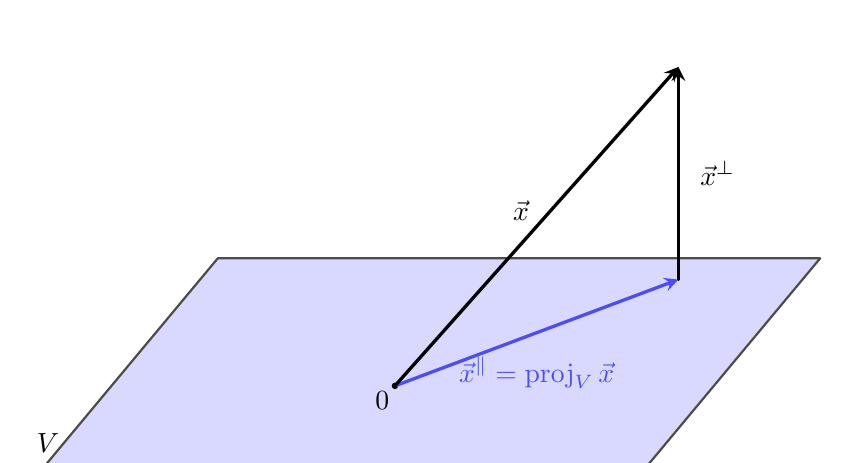
\begin{tikzpicture}[>=stealth, line cap=round, line join=round, scale=0.9]
  %--- Plane V (a tilted quadrilateral) ---
  \fill[blue!15] (-5,-1) -- (-2.5,2) -- (6,2) -- (3.5,-1) -- cycle;
  \draw[black!70, thick] (-5,-1) -- (-2.5,2) -- (6,2) -- (3.5,-1) -- cycle;
  \node[anchor=east] at (-4.6,-0.6) {$V$};

  %--- Origin on the plane ---
  \coordinate (O) at (0,0.2);
  \fill (O) circle (1.3pt);
  \node[below left=-2pt] at (O) {$0$};

  %--- Choose a projection point P on the plane and a vertical offset for x^\perp ---
  \coordinate (P) at (4,1.7);            % projection of x onto V
  \coordinate (X) at (4,4.7);            % tip of vector x (above the plane)

  %--- Vectors ---
  % x^{||} = proj_V x
  \draw[->, very thick, blue!70] (O) -- (P)
    node[midway, below=5pt] {$\vec x^{\parallel}=\mathrm{proj}_{V}\,\vec x$};

  % x^\perp (drawn "vertical" from the plane)
  \draw[->, very thick] (P) -- (X)
    node[midway, right=4pt] {$\vec x^{\perp}$};

  % x from origin to X
  \draw[->, very thick] (O) -- (X)
    node[pos=0.55, left=4pt] {$\vec x$};

\end{tikzpicture}
\end{center}

\end{prop}




\begin{thm}[Formula for the orthogonal projection]\label{thm:proj}
\
\\
If $V$ is a subspace of $\mathbb{R}^n$ with an \textbf{orthonormal basis} $\vec{u}_1, \ldots, \vec{u}_m$, then
\[
\operatorname{proj}_V \vec{x}=\vec{x}^{\|}=\left(\vec{u}_1 \cdot \vec{x}\right) \vec{u}_1+\cdots+\left(\vec{u}_m \cdot \vec{x}\right) \vec{u}_m .
\]
for all $\vec{x}$ in $\mathbb{R}^n$.
\end{thm}

\begin{warn}
The above is not true without an  \textbf{orthonormal basis}.
\end{warn}

\begin{defn}[Orthogonal complement]
\
\\
Consider a subspace $V$ of $\mathbb{R}^n$. The orthogonal complement $V^{\perp}$ of $V$ is the set of those vectors $\vec{x}$ in $\mathbb{R}^n$ that are orthogonal to all vectors in $V$ :
\[
V^{\perp}=\left\{\vec{x} \text { in } \mathbb{R}^n: \vec{v} \cdot \vec{x}=0, \text { for all } \vec{v} \text { in } V\right\}
\]
Note that $V^{\perp}$ is the kernel of the orthogonal projection onto $V$.
\end{defn}

\begin{thm}[Properties of the orthogonal complement]
\
\\
Consider a subspace $V$ of $\mathbb{R}^n$.\\
a. The orthogonal complement $V^{\perp}$ of $V$ is a subspace of $\mathbb{R}^n$.\\
b. The intersection of $V$ and $V^{\perp}$ consists of the zero vector: $V \cap V^{\perp}=\{\overrightarrow{0}\}$.\\
c. $\operatorname{dim}(V)+\operatorname{dim}\left(V^{\perp}\right)=n$.\\
d. $\left(V^{\perp}\right)^{\perp}=V$.
\end{thm}

\begin{prop}[Orthogonal Projection]
\
\\
If $Q$ has orthonormal columns spanning $S$, the orthogonal projector onto $S$ is $P=Q Q^\top$.
\end{prop}

\subsection{Gram--Schmidt Process}
\
\\


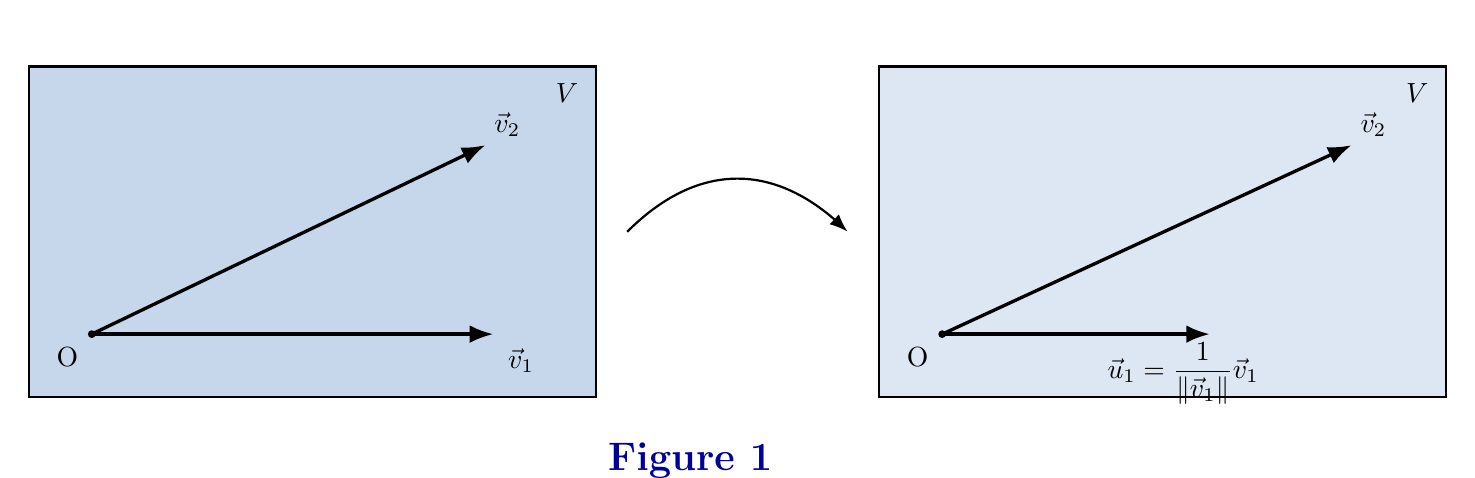
\begin{tikzpicture}
  % left panel
  \fill[panel] (0,0) rectangle (7.2,4.2);
  \draw[thick] (0,0) rectangle (7.2,4.2);
  \node[anchor=north east] at (7.1,4.1) {$V$};
  \fill (0.8,0.8) circle (1.4pt) node[below left=2pt]{O};
  \draw[vec] (0.8,0.8) -- (5.9,0.8) node[below right=2pt] {$\vec v_{1}$};
  \draw[vec] (0.8,0.8) -- (5.8,3.2) node[above right=-1pt] {$\vec v_{2}$};

  % arrow to right panel
  \draw[->,thick] (7.6,2.1) .. controls (8.5,3.0) and (9.5,3.0) .. (10.4,2.1);

  % right panel
  \begin{scope}[xshift=10.8cm]
    \fill[panel!60] (0,0) rectangle (7.2,4.2);
    \draw[thick] (0,0) rectangle (7.2,4.2);
    \node[anchor=north east] at (7.1,4.1) {$V$};
    \fill (0.8,0.8) circle (1.4pt) node[below left=2pt]{O};
\draw[vec] (0.8,0.8) -- (4.2,0.8)
  node[pos=0.9, below=-1pt] {$\vec u_{1}=\dfrac{1}{\|\vec v_{1}\|}\vec v_{1}$};
      \draw[vec] (0.8,0.8) -- (6.0,3.2) node[above right=-1pt] {$\vec v_{2}$};
  \end{scope}

  \node[blue!60!black, font=\bfseries\Large] at (8.4,-0.8) {Figure 1};
\end{tikzpicture}

% =========================
% Figure 2: v2 -> v2^|| + v2^\perp
% =========================
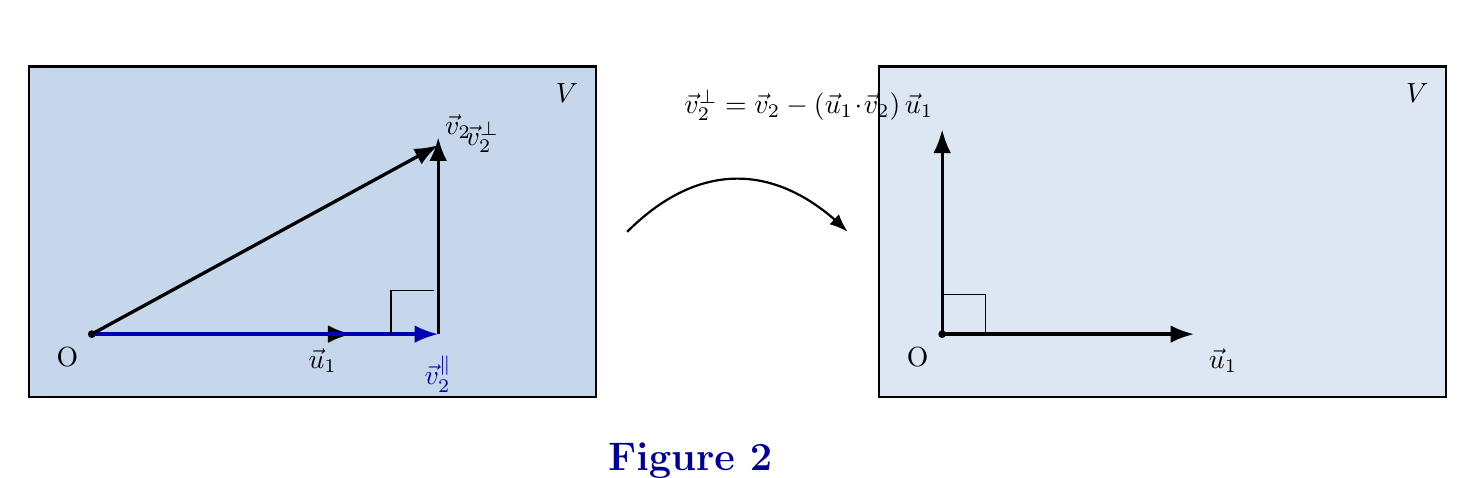
\begin{tikzpicture}
  % left panel
  \fill[panel] (0,0) rectangle (7.2,4.2);
  \draw[thick] (0,0) rectangle (7.2,4.2);
  \node[anchor=north east] at (7.1,4.1) {$V$};

  \fill (0.8,0.8) circle (1.4pt) node[below left=2pt]{O};
  \draw[vec] (0.8,0.8) -- (4.1,0.8) node[below left=2pt] {$\vec u_{1}$};

  % choose the projection point P and vertical tip
  \draw[vec,blue!70!black] (0.8,0.8) -- (5.2,0.8) node[below=4pt] {$\vec v_{2}^{\parallel}$};
  \draw[vec] (5.2,0.8) -- (5.2,3.3) node[below=3pt, right=6pt] {$\vec v_{2}^{\perp}$};
  % the original v2
  \draw[vec] (0.8,0.8) -- (5.2,3.2) node[above right=-2pt] {$\vec v_{2}$};
  % right angle box
  \draw (4.6,0.8) -- (4.6,1.35) -- (5.15,1.35);

  % arrow to right panel
  \draw[->,thick] (7.6,2.1) .. controls (8.5,3.0) and (9.5,3.0) .. (10.4,2.1);

  % right panel
  \begin{scope}[xshift=10.8cm]
    \fill[panel!60] (0,0) rectangle (7.2,4.2);
    \draw[thick] (0,0) rectangle (7.2,4.2);
    \node[anchor=north east] at (7.1,4.1) {$V$};

    \fill (0.8,0.8) circle (1.4pt) node[below left=2pt]{O};
    \draw[vec] (0.8,0.8) -- (0.8,3.4)
      node[above left=-1pt]
      {$\vec v_{2}^{\perp}=\vec v_{2}-(\vec u_{1}\!\cdot\!\vec v_{2})\,\vec u_{1}$};
    \draw[vec] (0.8,0.8) -- (4.0,0.8) node[below right=2pt] {$\vec u_{1}$};
\draw (0.8,0.8) -- (0.8,1.3) -- (1.35,1.3) -- (1.35,0.8);
  \end{scope}

  \node[blue!60!black, font=\bfseries\Large] at (8.4,-0.8) {Figure 2};
\end{tikzpicture}

% =========================
% Figure 3: normalize v2^\perp -> u2
% =========================
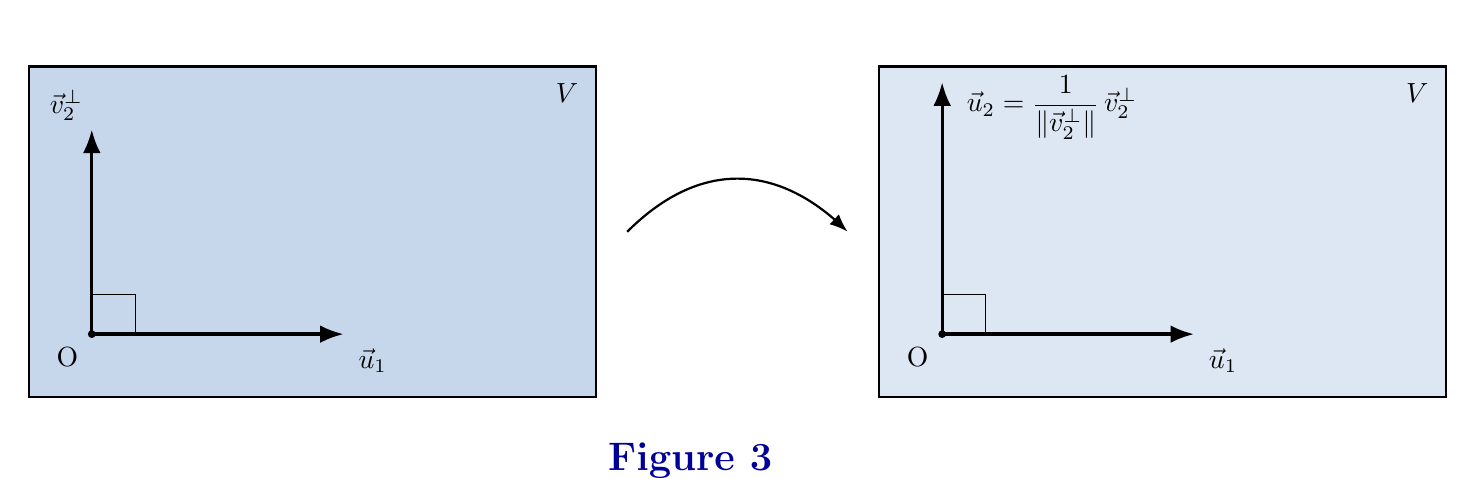
\begin{tikzpicture}
  % left
  \fill[panel] (0,0) rectangle (7.2,4.2);
  \draw[thick] (0,0) rectangle (7.2,4.2);
  \node[anchor=north east] at (7.1,4.1) {$V$};

  \fill (0.8,0.8) circle (1.4pt) node[below left=2pt]{O};
  \draw[vec] (0.8,0.8) -- (4.0,0.8) node[below right=2pt] {$\vec u_{1}$};
  \draw[vec] (0.8,0.8) -- (0.8,3.4) node[above left=-1pt] {$\vec v_{2}^{\perp}$};
\draw (0.8,0.8) -- (0.8,1.3) -- (1.35,1.3) -- (1.35,0.8);

  % arrow
  \draw[->,thick] (7.6,2.1) .. controls (8.5,3.0) and (9.5,3.0) .. (10.4,2.1);

  % right
  \begin{scope}[xshift=10.8cm]
    \fill[panel!60] (0,0) rectangle (7.2,4.2);
    \draw[thick] (0,0) rectangle (7.2,4.2);
    \node[anchor=north east] at (7.1,4.1) {$V$};

    \fill (0.8,0.8) circle (1.4pt) node[below left=2pt]{O};
    \draw[vec] (0.8,0.8) -- (4.0,0.8) node[below right=2pt] {$\vec u_{1}$};
    \draw[vec] (0.8,0.8) -- (0.8,4.0)
  node[pos=0.9, right=5pt] {$\vec u_{2}=\dfrac{1}{\|\vec v_{2}^{\perp}\|}\,\vec v_{2}^{\perp}$};
\draw (0.8,0.8) -- (0.8,1.3) -- (1.35,1.3) -- (1.35,0.8);
  \end{scope}

  \node[blue!60!black, font=\bfseries\Large] at (8.4,-0.8) {Figure 3};
\end{tikzpicture}


% Figure 4: Extension to 3D (corrected version)
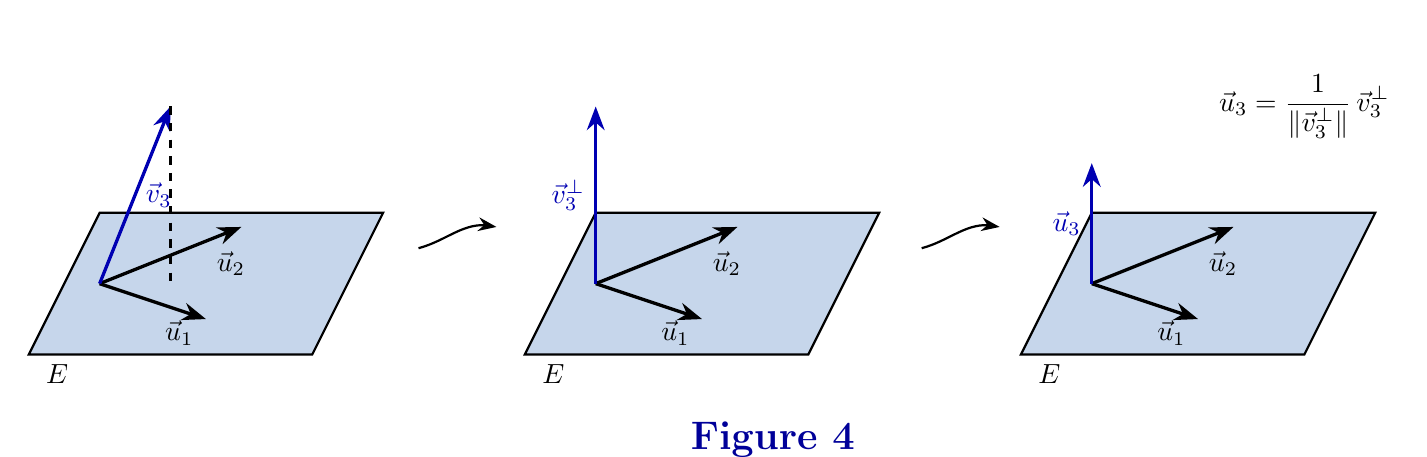
\begin{tikzpicture}[>=Stealth, thick, scale=0.9]
  \tikzset{vec/.style={very thick,-{Stealth[length=3mm]}}, ghost/.style={thick,dashed}}
  \definecolor{panel}{RGB}{198,214,235}

  % ---------- Left: v3 decomposition ----------
  \begin{scope}
    \fill[panel] (0,0) -- (4,0) -- (5,2) -- (1,2) -- cycle;
    \draw (0,0) -- (4,0) -- (5,2) -- (1,2) -- cycle;
    \node[anchor=north west] at (0.1,0) {$E$};

    % basis on the plane
    \draw[vec] (1,1) -- (2.5,0.5) node[near end, below] {$\vec u_1$};
        \draw[vec] (1,1) -- (3.0,1.8) node[near end, below right] {$\vec u_2$};


    % v3
    \draw[vec,blue!70!black] (1,1) -- (2,3.5) node[midway, right] {$\vec v_3$};
    % dashed projection (parallel to v3_perp, i.e. vertical)
    \draw[ghost] (2,3.5) -- (2,1); % now vertical, same as v3_perp
  \end{scope}

  % curved arrow to middle
  \draw[->,thick] (5.5,1.5) to[out=15,in=165] (6.6,1.8);

  % ---------- Middle: perpendicular component ----------
  \begin{scope}[shift={(7,0)}]
    \fill[panel] (0,0) -- (4,0) -- (5,2) -- (1,2) -- cycle;
    \draw (0,0) -- (4,0) -- (5,2) -- (1,2) -- cycle;
    \node[anchor=north west] at (0.1,0) {$E$};

    \draw[vec] (1,1) -- (2.5,0.5) node[near end, below] {$\vec u_1$};
    \draw[vec] (1,1) -- (3.0,1.8) node[near end, below right] {$\vec u_2$};
    % v3_perp stays vertical
    \draw[vec,blue!70!black] (1,1) -- (1,3.5) node[midway, left] {$\vec v_3^{\perp}$};
  \end{scope}

  % curved arrow to right
  \draw[->,thick] (12.6,1.5) to[out=15,in=165] (13.7,1.8);

  % ---------- Right: normalized u3 (shorter) ----------
  \begin{scope}[shift={(14,0)}]
    \fill[panel] (0,0) -- (4,0) -- (5,2) -- (1,2) -- cycle;
    \draw (0,0) -- (4,0) -- (5,2) -- (1,2) -- cycle;
    \node[anchor=north west] at (0.1,0) {$E$};

    \draw[vec] (1,1) -- (2.5,0.5) node[near end, below] {$\vec u_1$};
    \draw[vec] (1,1) -- (3.0,1.8) node[near end, below right] {$\vec u_2$};
    % shorter u3 to show unit norm
    \draw[vec,blue!70!black] (1,1) -- (1,2.7) node[midway, left] {$\vec u_3$};

    \node at (4,3.5)
      {$\displaystyle \vec u_3=\frac{1}{\|\vec v_3^{\perp}\|}\,\vec v_3^{\perp}$};
  \end{scope}

  \node[blue!60!black, font=\bfseries\Large] at (10.5,-1.2) {Figure 4};
\end{tikzpicture}

\begin{thm}[The Gram-Schmidt process]
\
\\
Consider a basis $\vec{v}_1, \ldots, \vec{v}_m$ of a subspace $V$ of $\mathbb{R}^n$. For $j=2, \ldots, m$, we resolve the vector $\vec{v}_j$ into its components parallel and perpendicular to the span of the preceding vectors, $\vec{v}_1, \ldots, \vec{v}_{j-1}$ :
\[
\vec{v}_j=\vec{v}_j^{\|}+\vec{v}_j^{\perp}, \quad \text { with respect to } \operatorname{span}\left(\vec{v}_1, \ldots, \vec{v}_{j-1}\right)
\]
Then
\[
\vec{u}_1=\frac{1}{\left\|\vec{v}_1\right\|} \vec{v}_1, \quad \vec{u}_2=\frac{1}{\left\|\vec{v}_2^{\perp}\right\|} \vec{v}_2^{\perp}, \ldots, \quad \vec{u}_j=\frac{1}{\left\|\vec{v}_j^{\perp}\right\|} \vec{v}_j^{\perp}, \ldots, \quad \vec{u}_m=\frac{1}{\left\|\vec{v}_m^{\perp}\right\|} \vec{v}_m^{\perp}
\]
is an orthonormal basis of $V$. By Theorem \ref{thm:proj}, we have
\[
\vec{v}_j^{\perp}=\vec{v}_j-\vec{v}_j^{\|}=\vec{v}_j-\left(\vec{u}_1 \cdot \vec{v}_j\right) \vec{u}_1-\cdots-\left(\vec{u}_{j-1} \cdot \vec{v}_j\right) \vec{u}_{j-1} .
\]
\end{thm}




\subsection{Orthogonal Transformations and Orthogonal Matrices}
\
\\
\begin{defn}[Orthogonal transformations and orthogonal matrices]
\
\\
A linear transformation $T$ from $\mathbb{R}^n$ to $\mathbb{R}^n$ is called orthogonal if it preserves the length of vectors:
\[
\|T(\vec{x})\|=\|\vec{x}\|, \quad \text { for all } \vec{x} \text { in } \mathbb{R}^n .
\]
If $T(\vec{x})=A \vec{x}$ is an orthogonal transformation, we say that $A$ is an orthogonal matrix.

Alternatively, a real $n\times n$ matrix
$Q$ is \textbf{orthogonal} if $Q^\top Q=I_n$. 
\end{defn}

\begin{thm}[]
\
\\
If $Q$ in an $n\times n$ orthogonal matrix, then $Q^{-1}=Q^\top$ and $\|Qx\|=\|x\|$; orthogonal maps preserve inner products and angles 9thus orthogonality).
\end{thm}

\begin{thm}[Orthogonal transformations and orthonormal bases]
\
\\
a. A linear transformation $T$ from $\mathbb{R}^n$ to $\mathbb{R}^n$ is orthogonal if (and only if) the vectors $T\left(\vec{e}_1\right), T\left(\vec{e}_2\right), \ldots, T\left(\vec{e}_n\right)$ form an orthonormal basis of $\mathbb{R}^n$.\\
b. An $n \times n$ matrix $A$ is orthogonal if (and only if) its columns form an orthonormal basis of $\mathbb{R}^n$.
\end{thm}



\begin{prop}[Products and inverses of orthogonal matrices]
\
\\
a. The product $A B$ of two orthogonal $n \times n$ matrices $A$ and $B$ is orthogonal.\\
b. The inverse $A^{-1}$ of an orthogonal $n \times n$ matrix $A$ is orthogonal.
\end{prop}


\begin{defn}[The transpose of a matrix; symmetric and skew-symmetric matrices]
\
\\
Consider an $m \times n$ matrix $A$.
The transpose $A^{\top} $ of $A$ is the $n \times m$ matrix whose $i j$ th entry is the $j i$ th entry of $A$ : The roles of rows and columns are reversed.

We say that a square matrix $A$ is symmetric if $A^{\top} =A$, and $A$ is called skew-symmetric if $A^{\top} =-A$.
\end{defn}

\begin{prop}
\
\\
If $\vec{v}$ and $\vec{w}$ are two (column) vectors in $\mathbb{R}^n$, then
\[
\begin{array}{cc}
\vec{v} \cdot \vec{w} & =\vec{v}^{\top}  \vec{w} \\
\uparrow & \uparrow \\
\text { Dot } & \text { Matrix } \\
\text { product } & \text { product }
\end{array}
\]
\end{prop}


\begin{prop}
\
\\
Consider an $n \times n$ matrix $A$. The matrix $A$ is orthogonal if (and only if) $A^{\top}  A= I_n$ or, equivalently, if $A^{-1}=A^{\top} $.
\end{prop}


\begin{thm}[The matrix of an orthogonal projection]\label{thm:orth-proj}
\
\\
Consider a subspace $V$ of $\mathbb{R}^n$ with orthonormal basis $\vec{u}_1, \vec{u}_2, \ldots, \vec{u}_m$. The matrix $P$ of the orthogonal projection onto $V$ is
\[
P=Q Q^{\top} , \quad \text { where } \quad Q=\left[\begin{array}{cccc}
\mid & \mid & & \mid \\
\vec{u}_1 & \vec{u}_2 & \ldots & \vec{u}_m \\
\mid & \mid & & \mid
\end{array}\right] \text {. }
\]
Pay attention to the order of the factors ( $Q Q^{\top} $ as opposed to $Q^{\top}  Q$ ). Note that matrix $P$ is symmetric, since $P^{\top} =\left(Q Q^{\top} \right)^{\top} =\left(Q^{\top} \right)^{\top}  Q^{\top} =Q Q^{\top} =P$.
\end{thm}

\begin{prop}[Orthogonal matrices summary]
\
\\
Consider an $n \times n$ matrix $A$. Then the following statements are equivalent:
\begin{itemize}
\item
 $A$ is an orthogonal matrix.
\item
The transformation $L(\vec{x})=A \vec{x}$ preserves length; that is, $\|A \vec{x}\|=\|\vec{x}\|$ for all $\vec{x}$ in $\mathbb{R}^n$.
\item
The columns of $A$ form an orthonormal basis of $\mathbb{R}^n$.
\item
$A^{\top}  A=I_n$.
\item
$A^{-1}=A^{\top} $.
\item
$A$ preserves the dot product, meaning that $(A \vec{x}) \cdot(A \vec{y})=\vec{x} \cdot \vec{y}$ for all $\vec{x}$ and $\vec{y}$ in $\mathbb{R}^n$.
\end{itemize}

\end{prop}

\subsection{Least Squares and Data Fitting}
\
\\

\begin{prop}[Image, Kernel and Transpose]
\
\\
For any matrix $A$,
\[
(\operatorname{im} A)^{\perp}=\operatorname{ker}\left(A^{\top} \right) .
\]
\end{prop}

\begin{prop}[A special case]
\
\\
If $A$ is an $n \times m$ matrix, then $\operatorname{ker}(A)=\operatorname{ker}\left(A^{\top}  A\right)$.\\
If $A$ is an $n \times m$ matrix with $\operatorname{ker}(A)=\{\overrightarrow{0}\}$, then $A^{\top}  A$ is invertible.
\end{prop}

\begin{prop}[An Alternative Characterization of Orthogonal Projections]
\
\\
Consider a vector $\vec{x}$ in $\mathbb{R}^n$ and a subspace $V$ of $\mathbb{R}^n$. Then the orthogonal projection $\operatorname{proj}_V \vec{x}$ is the vector in $V$ closest to $\vec{x}$, in that
\[
\left\|\vec{x}-\operatorname{proj}_V \vec{x}\right\|<\|\vec{x}-\vec{v}\|
\]
for all $\vec{v}$ in $V$ different from $\operatorname{proj}_V \vec{x}$.
\end{prop}

\begin{defn}[Least-squares solution]
\
\\
Consider a linear system
\[
A \vec{x}=\vec{b},
\]
where $A$ is an $n \times m$ matrix. A vector $\vec{x}^*$ in $\mathbb{R}^m$ is called a \textbf{least-squares solution} of this system if $\left\|\vec{b}-A \vec{x}^*\right\| \leq\|\vec{b}-A \vec{x}\|$ for all $\vec{x}$ in $\mathbb{R}^m$.
\end{defn}


\begin{thm}[Normal Equations]
\
\\
The least-squares solutions of the system

\[
A \vec{x}=\vec{b}
\]

are the exact solutions of the (consistent) system

\[
A^{\top}  A \vec{x}=A^{\top}  \vec{b} .
\]


The system $A^{\top}  A \vec{x}=A^{\top}  \vec{b}$ is called the \textbf{normal equation} of $A \vec{x}=\vec{b}$.

If $A$ has full column rank, the solution is unique.
\end{thm}


\begin{prop}[The matrix of an orthogonal projection]
\
\\
Consider a subspace $V$ of $\mathbb{R}^n$ with basis $\vec{v}_1, \vec{v}_2, \ldots, \vec{v}_m$. Let
\[
A=\left[\begin{array}{cccc}
\mid & \mid & & \mid \\
\vec{v}_1 & \vec{v}_2 & \ldots & \vec{v}_m \\
\mid & \mid & & \mid
\end{array}\right] .
\]
Then the matrix of the orthogonal projection onto $V$ is

\[
A\left(A^{\top}  A\right)^{-1} A^{\top}  .
\]
Note that we are not required to find an orthonormal basis of $V$ here, unlike in Theorem \ref{thm:orth-proj}.
\end{prop}
\subsection{Inner Product Spaces}
\
\\
\begin{defn}[Inner Product Space]
\
\\
An inner product in a linear space $V$ is a rule that assigns a real scalar (denoted by $\langle f, g\rangle$) to any pair $f, g$ of elements of $V$, such that the following properties hold for all $f, g, h$ in $V$, and all $c$ in $\mathbb{R}$ :\\
a. $\langle f, g\rangle=\langle g, f\rangle$ (symmetry).\\
b. $\langle f+h, g\rangle=\langle f, g\rangle+\langle h, g\rangle$.\\
c. $\langle c f, g\rangle=c\langle f, g\rangle$.\\
d. $\langle f, f\rangle>0$, for all nonzero $f$ in $V$ (positive definiteness).

A linear space endowed with an inner product is called an \textbf{inner product space}.
\end{defn}


\begin{defn}[Norm, orthogonality]
\
\\
The \textbf{norm} (or magnitude) of an element $f$ of an inner product space is
\[
\|f\|=\sqrt{\langle f, f\rangle} .
\]
Two elements $f$ and $g$ of an inner product space are called \textbf{orthogonal} (or \textbf{perpendicular}) if
\[
\langle f, g\rangle=0 .
\]
\end{defn}


\begin{thm}[Orthogonal projection]
\
\\
Similarly to Theorem \ref{thm:proj}, if $g_1, \ldots, g_m$ is an orthonormal basis of a subspace $W$ of an inner product space $V$, then
\[
\operatorname{proj}_W f=\left\langle g_1, f\right\rangle g_1+\cdots+\left\langle g_m, f\right\rangle g_m,
\]
for all $f$ in $V$.
\end{thm}


\section{Determinants}
\
\\
\subsection{Introduction to Determinants}
\
\\

\begin{defn}[Determinant of a $3 \times 3$ matrix, in terms of the columns] 
\
\\
If $A=\left[\begin{array}{lll}\vec{u} & \vec{v} & \vec{w}\end{array}\right]$, then
\[
\det A=\vec{u} \cdot(\vec{v} \times \vec{w}) .
\]
A $3 \times 3$ matrix $A$ is invertible if (and only if) $\det A \neq 0$.
\end{defn}

\begin{thm}[Sarrus's rule]
\
\\
To find the determinant of a $3 \times 3$ matrix $A$, write the first two columns of $A$ to the right of $A$. Then multiply the entries along the six diagonals shown below.\\
Add or subtract these diagonal products, as shown in the diagram:

\tikzset{node style ge/.style={circle}}
$\det(A)= \left|
\begin{matrix}
    a_{11} & a_{12} & a_{13}  \\
    a_{21} & a_{22} & a_{23}  \\
    a_{31} & a_{32} & a_{33}  \\
\end{matrix}%
\right|$
=$\big(a_{11}a_{22}a_{33}+a_{21}a_{32}a_{13}+a_{31}a_{12}a_{33}\big)-\big(a_{13}a_{22}a_{31}+a_{23}a_{32}a_{11}+a_{33}a_{12}a_{31}\big)$

\begin{center}


\begin{tikzpicture}[baseline=(A.center)]
  \tikzset{BarreStyle/.style =   {opacity=.4,line width=4 mm,line cap=round,color=#1}}
    \tikzset{SignePlus/.style =   {above left,inner sep=1.5pt,opacity=.4,circle,fill=#1}}
    \tikzset{SigneMoins/.style =   {below left,inner sep=-0.5pt,opacity=.4,circle,fill=#1}}
    \tikzset{PlusProduct/.style={anchor=north west,rectangle,rounded corners=5pt,inner sep=2pt,outer sep=2.5pt,opacity=.4,fill=#1}}
    \tikzset{MoinsProduct/.style={anchor=south west,rectangle,rounded corners=5pt,inner sep=2pt,outer sep=2.5pt,opacity=.4,fill=#1}}
% the matrices
\matrix (A) [matrix of math nodes, nodes = {node style ge},,column sep=0 mm] 
{ a_{11} & a_{12} & a_{13}  \\
  a_{21} & a_{22} & a_{23}  \\
  a_{31} & a_{32} & a_{33}  \\
  a_{11} & a_{12} & a_{13} \\
  a_{21} & a_{22} & a_{23}\\
};

 \draw [BarreStyle=blue] (A-1-1.north west) node[SignePlus=blue] {$+$} to (A-3-3.south east) node[PlusProduct=blue]{$a_{11}\times a_{22}\times a_{33}$};
 \draw [BarreStyle=blue] (A-2-1.north west) node[SignePlus=blue] {$+$} to (A-4-3.south east)  node[PlusProduct=blue]{$a_{21}\times a_{32}\times a_{13}$};
 \draw [BarreStyle=blue] (A-3-1.north west) node[SignePlus=blue] {$+$} to (A-5-3.south east)  node[PlusProduct=blue]{$a_{31}\times a_{12}\times a_{23}$};
 
 \draw [BarreStyle=red]  (A-3-1.south west) node[SigneMoins=red] {\strut $-$} to (A-1-3.north east) node[MoinsProduct=red]{$a_{31}\times a_{22}\times a_{13}$};
 \draw [BarreStyle=red]  (A-4-1.south west) node[SigneMoins=red] {\strut $-$} to (A-2-3.north east) node[MoinsProduct=red]{$a_{11}\times a_{32}\times a_{23}$};
 \draw [BarreStyle=red]  (A-5-1.south west) node[SigneMoins=red] {\strut $-$} to (A-3-3.north east) node[MoinsProduct=red]{$a_{21}\times a_{12}\times a_{33}$};
\end{tikzpicture}
\end{center}
\end{thm}



\begin{defn}[Determinant]
\
\\
$\det A$ is the alternating multilinear function of rows (or columns) normalized by $\det I=1$; equivalently by the Leibniz formula $\det A=\sum_{\sigma\in S_n} \operatorname{sgn}(\sigma)\prod_i a_{i,\sigma(i)}$.
\end{defn}


\begin{thm}[Determinant of a triangular matrix]
\
\\
The determinant of an (upper or lower) triangular matrix is the product of the diagonal entries of the matrix.

In particular, the determinant of a diagonal matrix is the product of its diagonal entries.
\end{thm}


\begin{thm}[Determinant of a block matrix]
\
\\
If $M=\left[\begin{array}{cc}A & B \\ 0 & C\end{array}\right]$, where $A$ and $C$ are square matrices (not necessarily of the same size), then
\[
\det \left[\begin{array}{cc}
A & B \\
0 & C
\end{array}\right]=(\det  A)(\det  C) .
\]
Likewise,
\[
\det \left[\begin{array}{ll}
A & 0 \\
B & C
\end{array}\right]=(\det  A)(\det  C) .
\]
\end{thm}



\subsection{Properties of the Determinant}
\
\\

\begin{thm}[Basic Properties]
\
\\
Row operations affect $\det$ as follows: 
\begin{itemize}
\item
swapping rows flips sign; 
\item 
scaling a row scales $\det$; 
\item
adding a multiple of one row to another leaves $\det$ unchanged;
\item
Also $\det(AB)=\det A\cdot\det B$.

\end{itemize}
\end{thm}

\begin{thm}[Determinant of the transpose]
\
\\
If $A$ is a square matrix, then
\[
\det \left(A^\top \right)=\det  A .
\]
\end{thm}


\begin{thm}[Linearity of the determinant in the rows and columns]
\
\\
Consider fixed row vectors $\vec{v}_1, \ldots, \vec{v}_{i-1}, \vec{v}_{i+1}, \ldots, \vec{v}_n$ with $n$ components. Then the function
\[
T(\vec{x})=\det \left[\begin{array}{ccc}
- & \vec{v}_1 & - \\
& \vdots & \\
- & \vec{v}_{i-1} & - \\
- & \vec{x} & - \\
- & \vec{v}_{i+1} & - \\
& \vdots & \\
- & \vec{v}_n & -
\end{array}\right] \quad \text { from } \mathbb{R}^{1 \times n} \text { to } \mathbb{R}
\]
is a linear transformation. This property is referred to as \textbf{linearity of the determinant in the $i$th row}. Likewise, the determinant is \textbf{linear in all the columns}.
\end{thm}


\begin{thm}[Elementary row operations and determinants]
\
\\
a. If $B$ is obtained from $A$ by dividing a row of $A$ by a scalar $k$, then $\det  B=(1 / k) \det  A$.\\
b. If $B$ is obtained from $A$ by a row swap, then
\[
\det  B=-\det  A .
\]
We say that the determinant is alternating on the rows.\\
c. If $B$ is obtained from $A$ by adding a multiple of a row of $A$ to another row, then
\[
\det  B=\det  A .
\]
Analogous results hold for elementary column operations.
\end{thm}

\begin{thm}[Invertibility and determinant]
\
\\
A square matrix $A$ is invertible if and only if $\det  A \neq 0$.
\end{thm}

\begin{thm}[Determinants of products and powers]
\
\\
If $A$ and $B$ are $n \times n$ matrices and $m$ is a positive integer, then\\
a. $\det (A B)=(\det  A)(\det  B)$, and\\
b. $\det \left(A^m\right)=(\det  A)^m$.
\end{thm}


\begin{thm}[Determinants of similar matrices]
\
\\
If matrix $A$ is similar to $B$, then $\det  A=\det  B$.
\end{thm}

\begin{warn}
The converse is not necessarily true. For instance 
Let
\(
A = I_2 = \begin{bmatrix} 1 & 0 \\ 0 & 1 \end{bmatrix},
B = \begin{bmatrix} 2 & 0 \\ 0 & \tfrac{1}{2} \end{bmatrix}.
\)
Then $\det(A)=\det(B)$.
However, $A$ and $B$ are not similar. 

Similar matrices must have the same eigenvalues (with the same algebraic multiplicities). Here
\[
\text{Spec}(A)=\{1,1\}, \qquad \text{Spec}(B)=\{2,\tfrac12\},
\]
so $A$ and $B$ do not have the same eigenvalues, and therefore cannot be similar.

\end{warn}


\begin{thm}[Determinant of an inverse]
\
\\
If $A$ is an invertible matrix, then
\[
\det \left(A^{-1}\right)=\frac{1}{\det  A}=(\det  A)^{-1} .
\]
\end{thm}

\subsection{Geometrical Interpretations; Cramer's Rule}
\
\\
\begin{prop}[Geometry and Cramer]
\
\\
$|\det A|$ equals the volume scaling of $x\mapsto Ax$. For invertible $A$, Cramer's rule gives $x_i=\dfrac{\det A_i}{\det A}$.
\end{prop}



\section{Eigenvalues and Eigenvectors}
\
\\
\subsection{Diagonalization}
\
\\
\begin{defn}[Diagonalizable Matrix]
\
\\
Consider a linear transformation $T(\vec{x})=A \vec{x}$ from $\mathbb{R}^n$ to $\mathbb{R}^n$. Then $A$ (or $T$ ) is said to be \textbf{diagonalizable} if the matrix $B$ of $T$ with respect to some basis is diagonal.

Equivalently, $A$ is \textbf{diagonalizable} if $A=SDS^{-1}$ with $D$ diagonal. From Definition \ref{similar}, this means $A$ is similar to $D$.

Equivalently there exists a basis of eigenvectors (called eigenbasis).
\end{defn}


\begin{defn}[Eigenvectors, eigenvalues, and eigenbases]
\
\\
Consider a linear transformation $T(\vec{x})=A \vec{x}$ from $\mathbb{R}^n$ to $\mathbb{R}^n$.
A \textbf{nonzero} vector $\vec{v}$ in $\mathbb{R}^n$ is called an \textbf{eigenvector} of $A$ (or $T$) if
\[
A \vec{v}=\lambda \vec{v}
\]
for some scalar $\lambda$. This $\lambda$ is called the \textbf{eigenvalue} associated with eigenvector $\vec{v}$.

A basis $\vec{v}_1, \ldots, \vec{v}_n$ of $\mathbb{R}^n$ is called an \textbf{eigenbasis} for $A$ (or $T$ ) if the vectors $\vec{v}_1, \ldots, \vec{v}_n$ are eigenvectors of $A$, meaning that $A \vec{v}_1=\lambda_1 \vec{v}_1, \ldots, A \vec{v}_n=\lambda_n \vec{v}_n$ for some scalars $\lambda_1, \ldots, \lambda_n$.
\end{defn}


\begin{thm}[Eigenbases and diagonalization]
\
\\
The matrix $A$ is diagonalizable if (and only if) there exists an eigenbasis for $A$. 

If $\vec{v}_1, \ldots, \vec{v}_n$ is an eigenbasis for $A$, with $A \vec{v}_1=\lambda_1 \vec{v}_1, \ldots, A \vec{v}_n=\lambda_n \vec{v}_n$, then the matrices
\[
S=\left[\begin{array}{cccc}
\mid & \mid & & \mid \\
\vec{v}_1 & \vec{v}_2 & \ldots & \vec{v}_n \\
\mid & \mid & & \mid
\end{array}\right] \text { and } B=\left[\begin{array}{cccc}
\lambda_1 & 0 & \ldots & 0 \\
0 & \lambda_2 & \ldots & 0 \\
\vdots & \vdots & \ddots & \vdots \\
0 & 0 & \ldots & \lambda_n
\end{array}\right]
\]
will diagonalize $A$, meaning that $S^{-1} A S=B$.

Conversely, if the matrices $S$ and $B$ diagonalize $A$, then the column vectors of $S$ will form an eigenbasis for $A$, and the diagonal entries of $B$ will be the associated eigenvalues.

\end{thm}

\begin{thm}[Eigenvalues of an orthogonal matrix]
\
\\
The possible \textbf{\textit{real}} eigenvalues of an orthogonal matrix are $1$ and $-1$ .
\end{thm}


\begin{thm}[Various characterizations of invertible matrices]
\
\\
For an $n \times n$ matrix $A$, the following statements are equivalent.
\begin{enumerate}[label=(\roman*)]
\item
$A$ is invertible.
\item
The linear system $A \vec{x} = \vec{b}$ has a unique solution $\vec{x}$, for all $\vec{b}$ in $\mathbb{R}^n$.
\item
 $\operatorname{rref} A=I_n$.
\item
$\operatorname{rank} A=n$.
\item
$\operatorname{im} A=\mathbb{R}^n$.
\item
$\ker A=\{\overrightarrow{0}\}$.
\item
The column vectors of $A$ form a basis of $\mathbb{R}^n$.
\item
The column vectors of $A$ span $\mathbb{R}^n$.
\item
The column vectors of $A$ are linearly independent.
\item
$\det  A \neq 0$.
\item
0 fails to be an eigenvalue of $A$.
\end{enumerate}
\end{thm}

\begin{thm}[Discrete dynamical systems]
\
\\
Consider the dynamical system
\[
\vec{x}(t+1)=A \vec{x}(t) \quad \text { with } \quad \vec{x}(0)=\vec{x}_0 .
\]
Then $\vec{x}(t)=A^\top \vec{x}_0$. Suppose we can find an eigenbasis $\vec{v}_1, \ldots, \vec{v}_n$ for $A$, with $A \vec{v}_1=\lambda_1 \vec{v}_1, \ldots, A \vec{v}_n=\lambda_n \vec{v}_n$. Find the coordinates $c_1, \ldots, c_n$ of the vector $\vec{x}_0$ with respect to the eigenbasis $\vec{v}_1, \ldots, \vec{v}_n$ :
\[
\vec{x}_0=c_1 \vec{v}_1+\cdots+c_n \vec{v}_n.
\]
Then
\[
\vec{x}(t)=A^\top \vec{x}_0=c_1 A^\top \vec{v}_1+\cdots+c_n A^\top \vec{v}_n=c_1 \lambda_1^\top \vec{v}_1+\cdots+c_n \lambda_n^\top \vec{v}_n.
\]
\end{thm}


\subsection{Finding the Eigenvalues of a Matrix}
\
\\

\begin{thm}[Characteristic Polynomial]
\
\\
If $A$ is an $n \times n$ matrix, then $\det \left(A-\lambda I_n\right)$ is a polynomial of degree $n$, of the form
\[
\begin{aligned}
& (-\lambda)^n+(\operatorname{tr} A)(-\lambda)^{n-1}+\cdots+\det  A \\
& \quad=(-1)^n \lambda^n+(-1)^{n-1}(\operatorname{tr} A) \lambda^{n-1}+\cdots+\det  A
\end{aligned}
\]
This is called the characteristic polynomial of $A$, denoted by $f_A(\lambda)$.

Some define the characteristic polynomial of $A$ as $\det \left(\lambda I_n  -A \right)$, which is a multiplication by $(-1)^n$.
\end{thm}

\begin{thm}[Eigenvalues and determinants; characteristic equation]
\
\\
Consider an $n \times n$ matrix $A$ and a scalar $\lambda$. Then $\lambda$ is an eigenvalue  of $A$ if and only if
\[
\det \left(A-\lambda I_n\right)=0
\]
This is called the characteristic equation (or the secular equation) of matrix $A$.
\end{thm}

\begin{defn}[Algebraic multiplicity of an eigenvalue]
\
\\
We say that an eigenvalue $\lambda_0$ of a square matrix $A$ has \textbf{algebraic multiplicity} $k$ if $\lambda_0$ is a root of multiplicity $k$ of the characteristic polynomial $f_A(\lambda)$, meaning that we can write
\[
f_A(\lambda)=\left(\lambda_0-\lambda\right)^k g(\lambda)
\]
for some polynomial $g(\lambda)$ with $g\left(\lambda_0\right) \neq 0$. We write $\operatorname{almu}(\lambda_0)=k$.
\end{defn}

\begin{thm}[Number of eigenvalues]
\
\\
An $n \times n$ matrix has at most $n$ real eigenvalues, even if they are counted with their algebraic multiplicities.

If $n$ is odd, then an $n \times n$ matrix has at least one real eigenvalue.
\end{thm}


\begin{thm}[Eigenvalues, determinant, and trace]
\
\\
If an $n \times n$ matrix $A$ has the eigenvalues $\lambda_1, \lambda_2, \ldots, \lambda_n$, listed with their algebraic multiplicities, then
\[
\det  A=\lambda_1 \lambda_2 \cdots \lambda_n, \quad \text { the product of the eigenvalues }
\]
and
\[
\operatorname{tr} A=\lambda_1+\lambda_2+\cdots+\lambda_n,  \quad \text { the sum of the eigenvalues.}
\]
\end{thm}


\subsection{Finding the Eigenvectors of a Matrix}
\
\\
\begin{defn}[Eigenspace]
\
\\
Consider an eigenvalue $\lambda$ of an $n \times n$ matrix $A$. Then the kernel of the matrix $A-\lambda I_n$ is called the \textbf{eigenspace} associated with $\lambda$, denoted by $E_\lambda$ :
\[
E_\lambda=\operatorname{ker}\left(A-\lambda I_n\right)=\left\{\vec{v} \text { in } \mathbb{R}^n: A \vec{v}=\lambda \vec{v}\right\} .
\]
\end{defn}


\begin{defn}[Geometric multiplicity]
\
\\
Consider an eigenvalue $\lambda$ of an $n \times n$ matrix $A$. The dimension of eigenspace $E_\lambda=\operatorname{ker}\left(A-\lambda I_n\right)$ is called the \textbf{geometric multiplicity} of eigenvalue $\lambda$, denoted $\operatorname{gemu}(\lambda)$. Thus,
\[
\operatorname{gemu}(\lambda)=\operatorname{nullity}\left(A-\lambda I_n\right)=n-\operatorname{rank}\left(A-\lambda I_n\right).
\]
\end{defn}

\begin{thm}[Eigenbases and geometric multiplicities]
\
\\
a. Consider an $n \times n$ matrix $A$. If we find a basis of each eigenspace of $A$ and concatenate all these bases, then the resulting eigenvectors $\vec{v}_1, \ldots, \vec{v}_s$ will be linearly independent. (Note that $s$ is the sum of the geometric multiplicities of the eigenvalues of $A$.) This result implies that $s \leq n$.

b. Matrix $A$ is diagonalizable if (and only if) the geometric multiplicities of the eigenvalues add up to $n$ (meaning that $s=n$ in part a).
\end{thm}

\begin{thm}[An $n \times n$ matrix with $n$ distinct eigenvalues]
\
\\
If an $n \times n$ matrix $A$ has $n$ distinct eigenvalues, then $A$ is diagonalizable. We can construct an eigenbasis by finding an eigenvector for each eigenvalue.
\end{thm}


\begin{thm}[The eigenvalues of similar matrices]
\
\\
Suppose matrix $A$ is similar to $B$. Then

a. Matrices $A$ and $B$ have the same characteristic polynomial; that is, $f_A(\lambda)=f_B(\lambda)$.

b. rank $A=\operatorname{rank} B$ and $\operatorname{nullity}A=\operatorname{nullity} B$.

c. Matrices $A$ and $B$ have the same eigenvalues, with the same algebraic and geometric multiplicities. (However, the eigenvectors need not be the same.)

d. Matrices $A$ and $B$ have the same determinant and the same trace: $\det  A=\det  B$ and $\operatorname{tr} A=\operatorname{tr} B$.
(However,  $A$ and $B$ have the same determinant and the same trace and not be similar.)
\end{thm}

\begin{thm}[Algebraic versus geometric multiplicity]
\
\\
If $\lambda$ is an eigenvalue of a square matrix $A$, then
\[
\operatorname{gemu}(\lambda) \leq \operatorname{almu}(\lambda) .
\]
\end{thm}



\begin{tech}[Strategy for Diagonalization]
\
\\
Suppose we are asked to determine whether a given $n \times n$ matrix $A$ is diagonalizable. If so, we wish to find an invertible matrix $S$ such that $S^{-1} A S=B$ is diagonal.

We can proceed as follows.

a. Find the eigenvalues of $A$ by solving the characteristic equation

\[
f_A(\lambda)=\det \left(A-\lambda I_n\right)=0 .
\]

b. For each eigenvalue $\lambda$, find a basis of the eigenspace

\[
E_\lambda=\operatorname{ker}\left(A-\lambda I_n\right) .
\]

c. Matrix $A$ is diagonalizable if (and only if) the dimensions of the eigenspaces add up to $n$. In this case, we find an eigenbasis $\vec{v}_1, \ldots, \vec{v}_n$
for $A$ by concatenating the bases of the eigenspaces we found in part b. Let

\[
S=\left[\begin{array}{cccc}
\mid & \mid & & \mid \\
\vec{v}_1 & \vec{v}_2 & \ldots & \vec{v}_n \\
\mid & \mid & & \mid
\end{array}\right] \text {. Then } S^{-1} A S=B=\left[\begin{array}{cccc}
\lambda_1 & 0 & \ldots & 0 \\
0 & \lambda_2 & \ldots & 0 \\
\vdots & \vdots & \ddots & \vdots \\
0 & 0 & \ldots & \lambda_n
\end{array}\right] \text {, }
\]

where $\lambda_j$ is the eigenvalue associated with $\vec{v}_j$.

\end{tech}

\begin{thm}[Cayley-Hamilton]\label{Cayley-Hamilton}
A square matrix satisfies its characteristic polynomial. 
That is 
\[
f_A(A)=0.
\]
\end{thm}

\subsection{More on Dynamical Systems}
\
\\
\begin{prop}[Discrete Linear Systems]
\
\\
For $x_{k+1}=Ax_k$, solutions are combinations of $\lambda_i^k v_i$ along eigen-directions; stability depends on $|\lambda_i|$.
\end{prop}


\begin{thm}[Powers of a diagonalizable matrix]
\
\\
If
\[
S^{-1} A S=B=\left[\begin{array}{cccc}
\lambda_1 & 0 & \ldots & 0 \\
0 & \lambda_2 & \ldots & 0 \\
\vdots & \vdots & \ddots & \vdots \\
0 & 0 & \ldots & \lambda_n
\end{array}\right]
\]
then
\[
A^\top=S B^\top S^{-1}=S\left[\begin{array}{cccc}
\lambda_1^\top & 0 & \ldots & 0 \\
0 & \lambda_2^\top & \ldots & 0 \\
\vdots & \vdots & \ddots & \vdots \\
0 & 0 & \ldots & \lambda_n^\top
\end{array}\right] S^{-1}
\]
\end{thm}


\subsection{Complex Eigenvalues}
\
\\
\begin{thm}[Fundamental theorem of algebra]
\
\\
Any polynomial $p(\lambda)$ with complex coefficients splits; that is, it can be written as a product of linear factors
\[
p(\lambda)=k\left(\lambda-\lambda_1\right)\left(\lambda-\lambda_2\right) \cdots\left(\lambda-\lambda_n\right),
\]
for some complex numbers $\lambda_1, \lambda_2, \ldots, \lambda_n$, and $k$. (The $\lambda_i$ need not be distinct.)
Therefore, a polynomial $p(\lambda)$ of degree $n$ has precisely $n$ complex roots if they are properly counted with their multiplicities.
\end{thm}


\begin{prop}[Complex Pairs]
\
\\
Real matrices may have complex conjugate eigenpairs; real dynamics then mix rotations and scalings.
\end{prop}


\begin{thm}[]
\
\\
For a $2\times 2$ matrix $A$ with complex eigenvalues $\lambda = \alpha \pm i\beta$, the matrix exponential is given by the formula:
\[
 e^{At} = e^{\alpha t} \left( \cos(\beta t) I_2 + \frac{\sin(\beta t)}{\beta} (A - \alpha I_2) \right).
 \]
One proof uses Cayley-Hamilton's theorem, \ref{Cayley-Hamilton}.
\end{thm}

\subsection{Stability}
\
\\
\begin{defn}[Stability Criteria/Equilibrium]
\
\\
Consider a dynamical system
\[
\vec{x}(t+1)=A \vec{x}(t) .
\]
We say that $\overrightarrow{0}$ is an (asymptotically) stable equilibrium for this system if
\[
\lim _{t \rightarrow \infty} \vec{x}(t)=\lim _{t \rightarrow \infty}\left(A^t \vec{x}_0\right)=\overrightarrow{0}
\]
for all vectors $\vec{x}_0$ in $\mathbb{R}^n$.
\end{defn}


\begin{thm}[Stability and eigenvalues]
\
\\
Consider a dynamical system $\vec{x}(t+1)=A \vec{x}(t)$. The zero state is asymptotically stable if (and only if) the modulus of all the complex eigenvalues of $A$ is less than $1$.
\end{thm}

\begin{thm}[Dynamical systems with complex eigenvalues]
\
\\
Consider the dynamical system $\vec{x}(t+1)=A \vec{x}(t)$, where $A$ is a real $2 \times 2$ matrix with eigenvalues
\[
\lambda_{1,2}=p \pm i q=r(\cos (\theta) \pm i \sin (\theta)), \quad \text { where } \quad q \neq 0 .
\]
Let $\vec{v}+i \vec{w}$ be an eigenvector of $A$ with eigenvalue $p+i q$.
Then
\[
\vec{x}(t)=r^t S\left[\begin{array}{rr}
\cos (\theta t) & -\sin (\theta t) \\
\sin (\theta t) & \cos (\theta t)
\end{array}\right] S^{-1} \vec{x}_0, \quad \text { where } \quad S=\left[\begin{array}{ll}
\vec{w} & \vec{v}
\end{array}\right] .
\]


Note that $S^{-1} \vec{x}_0$ is the coordinate vector of $\vec{x}_0$ with respect to basis $\vec{w}, \vec{v}$.
\end{thm}

\begin{thm}[Phase portrait of a system with complex eigenvalues
]
\
\\
Consider a dynamical system
\[
\vec{x}(t+1)=A \vec{x}(t),
\]
where $A$ is a real $2 \times 2$ matrix with eigenvalues $\lambda_{1,2}=p \pm i q$ (where $q \neq 0$ ). Let
\[
r=\left|\lambda_1\right|=\left|\lambda_2\right|=\sqrt{p^2+q^2}
\]
If $r=1$, then the points $\vec{x}(t)$ are located on an ellipse; if $r$ exceeds 1 , then the trajectory spirals outward; and if $r$ is less than 1 , then the trajectory spirals inward, approaching the origin.
\end{thm}



\section{Symmetric Matrices and Quadratic Forms}
\
\\


\subsection{Symmetric Matrices}
\
\\
\begin{thm}[Spectral Theorem]
\
\\
A matrix $A$ is orthogonally diagonalizable (i.e., there exists an orthogonal $S$ such that $S^{-1} A S=S^\top A S$ is diagonal) if and only if $A$ is symmetric (i.e., $\left.A^\top=A\right)$.
\end{thm}


\begin{thm}
\
\\
Consider a symmetric matrix $A$. If $\vec{v}_1$ and $\vec{v}_2$ are eigenvectors of $A$ with distinct eigenvalues $\lambda_1$ and $\lambda_2$, then $\vec{v}_1 \cdot \vec{v}_2=0$; that is, $\vec{v}_2$ is orthogonal to $\vec{v}_1$.
\end{thm}


\begin{thm}
\
\\
A symmetric $n \times n$ matrix $A$ has $n$ real eigenvalues if they are counted with their algebraic multiplicities.
\end{thm}

\begin{thm}
Orthogonal diagonalization of a symmetric matrix $A$\\
a. Find the eigenvalues of $A$, and find a basis of each eigenspace.\\
b. Using the Gram-Schmidt process, find an orthonormal basis of each eigenspace.\\
c. Form an orthonormal eigenbasis $\vec{v}_1, \vec{v}_2, \ldots, \vec{v}_n$ for $A$ by concatenating the orthonormal bases you found in part b, and let
\[
S=\left[\begin{array}{cccc}
\mid & \mid & & \mid \\
\vec{v}_1 & \vec{v}_2 & \ldots & \vec{v}_n \\
\mid & \mid & & \mid
\end{array}\right] .
\]
$S$ is orthogonal, and $S^{-1} A S$ will be diagonal.
\end{thm}



\subsection{Quadratic Forms}
\
\\
\begin{defn}[Quadratic Forms]
\
\\
A function $q\left(x_1, x_2, \ldots, x_n\right)$ from $\mathbb{R}^n$ to $\mathbb{R}$ is called a \textbf{quadratic form} if it is a linear combination of functions of the form $x_i x_j$ (where $i$ and $j$ may be equal). A quadratic form can be written as
\[
q(\vec{x})=\vec{x} \cdot A \vec{x}=\vec{x}^\top A \vec{x}
\]
for a unique symmetric $n \times n$ matrix $A$, called the matrix of $q$.
\end{defn}


\begin{thm}[Diagonalizing a quadratic form]
\
\\
Consider a quadratic form $q(\vec{x})=\vec{x} \cdot A \vec{x}$, where $A$ is a symmetric $n \times n$ matrix. Let $\mathfrak{B}$ be an orthonormal eigenbasis for $A$, with associated eigenvalues $\lambda_1, \ldots, \lambda_n$. Then
\[
q(\vec{x})=\lambda_1 c_1^2+\lambda_2 c_2^2+\cdots+\lambda_n c_n^2,
\]
where the $c_i$ are the coordinates of $\vec{x}$ with respect to $\mathfrak{B} .^2$
\end{thm}


\begin{defn}[Definiteness of a quadratic form]
\
\\
Consider a quadratic form $q(\vec{x})=\vec{x} \cdot A \vec{x}$, where $A$ is a symmetric $n \times n$ matrix.
We say that $A$ is \textbf{positive definite} if $q(\vec{x})$ is positive for all nonzero $\vec{x}$ in $\mathbb{R}^n$, and we call $A$ \textbf{positive semidefinite} if $q(\vec{x}) \geq 0$, for all $\vec{x}$ in $\mathbb{R}^n$.

Negative definite and negative semidefinite symmetric matrices are defined analogously.

Finally, we call $A$ indefinite if $q$ takes positive as well as negative values.
\end{defn}



\begin{thm}[Eigenvalues and definiteness]
\
\\
A symmetric matrix $A$ is positive definite if (and only if) all of its eigenvalues are positive. The matrix $A$ is positive semidefinite if (and only if) all of its eigenvalues are positive or zero.
\end{thm}

\begin{thm}[Principal submatrices and definiteness]
\
\\
Consider a symmetric $n \times n$ matrix $A$. For $m=1, \ldots, n$, let $A^{(m)}$ be the $m \times m$ matrix obtained by omitting all rows and columns of $A$ past the $m$-th. These matrices $A^{(m)}$ are called the principal submatrices of $A$.

The matrix $A$ is positive definite if (and only if) $\det \left(A^{(m)}\right)>0$, for all $m=1, \ldots, n$.
\end{thm}

\begin{defn}[Principal axes]
\
\\
Consider a quadratic form $q(\vec{x})=\vec{x} \cdot A \vec{x}$, where $A$ is a symmetric $n \times n$ matrix with $n$ distinct eigenvalues. Then the eigenspaces of $A$ are called the \textbf{principal axes} of $q$. (Note that these eigenspaces will be one-dimensional.)
\end{defn}


\begin{thm}[Ellipses and hyperbolas]
\
\\
Consider the curve $C$ in $\mathbb{R}^2$ defined by
\[
q\left(x_1, x_2\right)=a x_1^2+b x_1 x_2+c x_2^2=1 .
\]
Let $\lambda_1$ and $\lambda_2$ be the eigenvalues of the matrix $\begin{bmatrix}a & b / 2 \\ b / 2 & c\end{bmatrix}$ of $q$.\\
If both $\lambda_1$ and $\lambda_2$ are positive, then $C$ is an \textbf{ellipse}. \\
If one eigenvalue is positive and the other is negative, then $C$ is a \textbf{hyperbola}.
\end{thm}

\subsection{Singular Values}
\
\\

\begin{defn}[Singular values]
\
\\
The singular values of an $n \times m$ matrix $A$ are the square roots of the eigenvalues of the symmetric $m \times m$ matrix $A^{\top}  A$, listed with their algebraic multiplicities. It is customary to denote the singular values by $\sigma_1, \sigma_2, \ldots, \sigma_m$ and to list them in decreasing order:
\[
\sigma_1 \geq \sigma_2 \geq \cdots \geq \sigma_m \geq 0
\]
\end{defn}


\begin{thm}[Singular Value Decomposition]
\
\\
For any $A\in\mathbb{R}^{m\times n}$, $A=U\Sigma V^\top$ with $U,V$ orthogonal and $\Sigma=\operatorname{diag}(\sigma_i)$, $\sigma_i\ge 0$. Moreover $\sigma_i=\sqrt{\lambda_i(A^\top A)}$.
\end{thm}

\section{Linear Differential Equations}
\
\\
\subsection{An Introduction to Continuous Dynamical Systems}
\
\\

\begin{thm}[Exponential growth and decay]
\
\\
Consider the linear differential equation
\[
\frac{d x}{d t}=k x
\]
with initial value $x_0$ ( $k$ is an arbitrary constant). The solution is
\[
x(t)=e^{k t} x_0 .
\]
The quantity $x$ will grow or decay exponentially (depending on the sign of $k$).
\end{thm}


\begin{thm}[Linear dynamical systems: Discrete versus continuous]
\
\\
A linear dynamical system can be modeled by
\[
\vec{x}(t+1)=B \vec{x}(t) \quad(\text { discrete model })
\]
or
\[
\frac{d \vec{x}}{d t}=A \vec{x} \quad \text { (continuous model) }
\]
$A$ and $B$ are $n \times n$ matrices, where $n$ is the number of components of the system.
\end{thm}


\begin{thm}[Continuous dynamical systems] \label{thm:dynamic-sys}
\
\\
Consider the system $d \vec{x} / d t=A \vec{x}$. Suppose there is a real eigenbasis $\vec{v}_1, \ldots, \vec{v}_n$ for $A$, with associated eigenvalues $\lambda_1, \ldots, \lambda_n$. Then the general solution of the system is
\[
\vec{x}(t)=c_1 e^{\lambda_1 t} \vec{v}_1+\cdots+c_n e^{\lambda_n t} \vec{v}_n
\]
The scalars $c_1, c_2, \ldots, c_n$ are the coordinates of $\vec{x}_0$ with respect to the basis $\vec{v}_1, \vec{v}_2, \ldots, \vec{v}_n$.

We can write the preceding equation in matrix form as

\[
\begin{aligned}
& \vec{x}(t)=\left[\begin{array}{cccc}
\mid & \mid & & \mid \\
\vec{v}_1 & \vec{v}_2 & \ldots & \vec{v}_n \\
\mid & \mid & & \mid
\end{array}\right]\left[\begin{array}{cccc}
e^{\lambda_1 t} & 0 & \cdots & 0 \\
0 & e^{\lambda_2 t} & \cdots & 0 \\
\vdots & \vdots & \ddots & \vdots \\
0 & 0 & \cdots & e^{\lambda_n t}
\end{array}\right]\left[\begin{array}{c}
c_1 \\
c_2 \\
\vdots \\
c_n
\end{array}\right] \\
& =S\left[\begin{array}{cccc}
e^{\lambda_1 t} & 0 & \cdots & 0 \\
0 & e^{\lambda_2 t} & \cdots & 0 \\
\vdots & \vdots & \ddots & \vdots \\
0 & 0 & \cdots & e^{\lambda_n t}
\end{array}\right] S^{-1} \vec{x}_0,
\end{aligned}
\]
where $S=\left[\begin{array}{cccc}
\mid & \mid & & \mid \\
\vec{v}_1 & \vec{v}_2 & \cdots & \vec{v}_n \\
\mid & \mid&  & \mid
\end{array}\right]$.

\end{thm}

\begin{defn}[Matrix Exponential]
\
\\
For $\dot{x}=Ax$, the solution is $x(t)=e^{tA}x(0)$ with $e^{tA}=\sum_{k\ge 0}\frac{t^k}{k!}A^k$.
\end{defn}

\subsection{The Complex Case: Euler's Formula}
\
\\
\begin{thm}[Euler]
\
\\
$e^{i\theta}=\cos\theta+i\sin\theta$. Complex eigenpairs produce oscillatory real solutions via real/imag parts.
\end{thm}


\begin{thm}[Continuous dynamical systems with complex eigenvalues]
\
\\
Consider a linear system
\[
\frac{d \vec{x}}{d t}=A \vec{x} .
\]
Suppose there exists a complex eigenbasis $\vec{v}_1, \ldots, \vec{v}_n$ for $A$, with associated complex eigenvalues $\lambda_1, \ldots, \lambda_n$. Then the general complex solution of the system is
\[
\vec{x}(t)=c_1 e^{\lambda_1 t} \vec{v}_1+\cdots+c_n e^{\lambda_n t} \vec{v}_n,
\]
where the $c_i$ are arbitrary complex numbers.

We can write this solution in matrix form, as in Theorem \ref{thm:dynamic-sys}
\end{thm}


\begin{thm}[Stability of a continuous dynamical system]
\
\\
For a system
\[
\frac{d \vec{x}}{d t}=A \vec{x},
\]
the zero state is an asymptotically stable equilibrium solution if (and only if) the real parts of all eigenvalues of $A$ are negative.
\end{thm}

\begin{thm}[Determinant, trace, and stability]
\
\\
Consider the system
\[
\frac{d \vec{x}}{d t}=A \vec{x}
\]
where $A$ is a real $2 \times 2$ matrix. Then the zero state is an asymptotically stable equilibrium solution if (and only if) $\operatorname{tr} A<0$ and $\det  A>0$.
\end{thm}



\begin{thm}[Continuous dynamical systems with eigenvalues $p \pm i q$]
\
\\
Consider the linear system
\[
\frac{d \vec{x}}{d t}=A \vec{x},
\]
where $A$ is a real $2 \times 2$ matrix with complex eigenvalues $p \pm i q$ (and $q \neq 0$ ). Consider an eigenvector $\vec{v}+i \vec{w}$ with eigenvalue $p+i q$. Then
\[
\vec{x}(t)=e^{p t} S\left[\begin{array}{rr}
\cos (q t) & -\sin (q t) \\
\sin (q t) & \cos (q t)
\end{array}\right] S^{-1} \vec{x}_0,
\]
where $S=\left[\begin{array}{ll}\vec{w} & \vec{v}\end{array}\right]$. Recall that $S^{-1} \vec{x}_0$ is the coordinate vector of $\vec{x}_0$ with respect to basis $\vec{w}, \vec{v}$.

The trajectories are either ellipses (linearly distorted circles), if $p=0$, or spirals, spiraling outward if $p$ is positive and inward if $p$ is negative. In the case of an ellipse, the trajectories have a period of $2 \pi / q$.
\end{thm}


\subsection{Linear Differential Operators and Linear Differential Equations}
\
\\
\begin{defn}[Linear differential operators and linear differential equations]
\
\\
A transformation $T$ from $C^{\infty}$ to $C^{\infty}$ of the form
\[
T(f)=f^{(n)}+a_{n-1} f^{(n-1)}+\cdots+a_1 f^{\prime}+a_0 f
\]
is called an $n$th-order \textbf{linear differential operator}. Here $f^{(k)}$ denotes the $k$th derivative of function $f$, and the coefficients $a_k$ are complex scalars.

If $T$ is an $n$th-order linear differential operator and $g$ is a smooth function, then the equation
\[
T(f)=g \quad \text { or } \quad f^{(n)}+a_{n-1} f^{(n-1)}+\cdots+a_1 f^{\prime}+a_0 f=g
\]
is called an $n$th-order \textbf{linear differential equation} (DE). The DE is called \textbf{homogeneous} if $g=0$ and \textbf{inhomogeneous} otherwise.
\end{defn}

\begin{thm}
\
\\
Consider a linear transformation $T$ from $V$ to $W$, where $V$ and $W$ are arbitrary linear spaces. Suppose we have a basis $f_1, f_2, \ldots, f_n$ of the kernel of $T$. Consider an equation $T(f)=g$ with a particular solution $f_p$. Then the solutions $f$ of the equation $T(f)=g$ are of the form
\[
f=c_1 f_1+c_2 f_2+\cdots+c_n f_n+f_p,
\]
where the $c_i$ are arbitrary constants.
\end{thm}

\begin{thm}
\
\\
The kernel of an $n$th-order linear differential operator is $n$-dimensional.
\end{thm}

\begin{tech}[Strategy for solving linear differential equations]\label{tech:lin}
\
\\
To solve an $n$th-order linear DE
\(
T(f)=g,
\)
we have to find\\
a. a basis $f_1, \ldots, f_n$ of $\operatorname{ker}(T)$, and\\
b. a particular solution $f_p$ of the DE $T(f)=g$.

Then the solutions $f$ are of the form
\[
f=c_1 f_1+\cdots+c_n f_n+f_p,
\]
where the $c_i$ are arbitrary constants.
\end{tech}


\begin{defn}[Eigenfunctions]
\
\\
Consider a linear differential operator $T$ from $C^{\infty}$ to $C^{\infty}$. A smooth function $f$ is called an \textbf{eigenfunction} of $T$ if $T(f)=\lambda f$ for some complex scalar $\lambda$; this scalar $\lambda$ is called the eigenvalue associated with the eigenfunction $f$.
\end{defn}


\begin{defn}[Characteristic polynomial]
\
\\
Consider the linear differential operator
\[
T(f)=f^{(n)}+a_{n-1} f^{(n-1)}+\cdots+a_1 f^{\prime}+a_0 f
\]
The \textbf{characteristic polynomial} of $T$ is defined as
\[
p_T(\lambda)=\lambda^n+a_{n-1} \lambda^{n-1}+\cdots+a_1 \lambda+a_0 .
\]
\end{defn}
\begin{thm}
\
\\
If $T$ is a linear differential operator, then $e^{\lambda t}$ is an eigenfunction of $T$, with associated eigenvalue $p_T(\lambda)$, for all $\lambda$ :
\[
T\left(e^{\lambda t}\right)=p_T(\lambda) e^{\lambda t} .
\]
In particular, if $p_T(\lambda)=0$, then $e^{\lambda t}$ is in the kernel of $T$.
\end{thm}


\begin{thm}[The kernel of a linear differential operator]\label{thm:kernel}
\
\\
Consider an $n$th-order linear differential operator $T$ whose characteristic polynomial $p_T(\lambda)$ has $n$ distinct roots $\lambda_1, \ldots, \lambda_n$. Then the exponential functions
\[
e^{\lambda_1 t}, e^{\lambda_2 t}, \ldots, e^{\lambda_n t}
\]
form a basis of the kernel of $T$; that is, they form a basis of the solution space of the homogeneous DE
\[
T(f)=0 .
\]
\end{thm}


\begin{thm}[With Complex Roots]
\
\\
Consider a differential equation
\[
T(f)=f^{\prime \prime}+a f^{\prime}+b f=0,
\]
where the coefficients $a$ and $b$ are real. Suppose the zeros of $p_T(\lambda)$ are $p \pm i q$, with $q \neq 0$. Then the solutions of the given DE are
\[
f(t)=e^{p t}\left(c_1 \cos (q t)+c_2 \sin (q t)\right),
\]
where $c_1$ and $c_2$ are arbitrary constants.
The special case when $a=0$ and $b>0$ is important in many applications. Then $p=0$ and $q=\sqrt{b}$, so that the solutions of the DE
\[
f^{\prime \prime}+b f=0
\]
are
\[
f(t)=c_1 \cos (\sqrt{b} t)+c_2 \sin (\sqrt{b} t) .
\]
\end{thm}

\begin{thm}
\
\\
Recall the notation $D f=f^{\prime}$ for the derivative operator. 

We let
\(
D^m=\underbrace{D \circ D \circ \cdots \circ D}_{m \text { times }};
\)
that is,
\(
D^m f=f^{(m)}.
\)
Then the operator
\[
T(f)=f^{(n)}+a_{n-1} f^{(n-1)}+\cdots+a_1 f^{\prime}+a_0 f
\]
can be written more succinctly as
\[
T=D^n+a_{n-1} D^{n-1}+\cdots+a_1 D+a_0,
\]
the characteristic polynomial $p_T(\lambda)$ ``evaluated at $D$".

An $n$ th-order linear differential operator $T$ can be expressed as the composite of $n$ first-order linear differential operators:
\[
\begin{aligned}
T & =D^n+a_{n-1} D^{n-1}+\cdots+a_1 D+a_0 \\
& =\left(D-\lambda_1\right)\left(D-\lambda_2\right) \cdots\left(D-\lambda_n\right)
\end{aligned}
\]
where the $\lambda_i$ are complex numbers.


\end{thm}

\begin{thm}
\
\\
Consider the linear differential equation
\[
f^{\prime \prime}(t)+a f^{\prime}(t)+b f(t)=C \cos (\omega t)
\]
where $a, b, C$, and $\omega$ are real numbers. Suppose that $a \neq 0$ or $b \neq \omega^2$. This DE has a particular solution of the form
\[
f_p(t)=P \cos (\omega t)+Q \sin (\omega t)
\]
Now use Technics \ref{tech:lin} and Theorems \ref{thm:kernel} to find all solutions $f$ of the DE.
\end{thm}

\begin{tech}[Strategy for linear differential equations]
\
\\
Suppose you have to solve an $n$ th-order linear differential equation $T(f)=g$.\\
\textbf{Step 1} Find $n$ linearly independent solutions of the DE $T(f)=0$.
\begin{itemize}
\item
Write the characteristic polynomial $p_T(\lambda)$ of $T$ [replacing $f^{(k)}$ by $\lambda^k$ ].
\item
Find the solutions $\lambda_1, \lambda_2, \ldots, \lambda_n$ of the equation $p_T(\lambda)=0$.
\item
If $\lambda$ is a solution of the equation $p_T(\lambda)=0$, then $e^{\lambda t}$ is a solution of $T(f)=$ 0 .
\item
If $\lambda$ is a solution of $p_T(\lambda)=0$ with multiplicity $m$, then $e^{\lambda t}, t e^{\lambda t}, t^2 e^{\lambda t}, \ldots$, $t^{m-1} e^{\lambda t}$ are solutions of the DE $T(f)=0$.% See Exercise 38.
\item
If $p \pm i q$ are complex solutions of $p_T(\lambda)=0$, then $e^{p t} \cos (q t)$ and $e^{p t} \sin (q t)$ are real solutions of the DE $T(f)=0$.
\end{itemize}

\textbf{Step 2} If the DE is inhomogeneous (i.e., if $g \neq 0$ ), find one particular solution $f_p$ of the $\operatorname{DE} T(f)=g$.
\begin{itemize}
\item
If $g$ is of the form $g(t)=A \cos (\omega t)+B \sin (\omega t)$, look for a particular solution of the same form, $f_p(t)=P \cos (\omega t)+Q \sin (\omega t)$.
\item
If $g$ is constant, look for a constant particular solution $f_p(t)=c .^7$
\item
If the DE is of first order, of the form $f^{\prime}(t)-a f(t)=g(t)$, use the formula $f(t)=e^{a t} \int e^{-a t} g(t) d t$.
\item
If none of the preceding techniques applies, write $T=\left(D-\lambda_1\right) \left(D-\lambda_2\right) \cdots\left(D-\lambda_n\right)$, and solve the corresponding first-order DEs.
\end{itemize}
\textbf{Step 3} The solutions of the $\operatorname{DE} T(f)=g$ are of the form
\[
f(t)=c_1 f_1(t)+c_2 f_2(t)+\cdots+c_n f_n(t)+f_p(t)
\]
where $f_1, f_2, \ldots, f_n$ are the solutions from step 1 and $f_p$ is the solution from step 2.
\end{tech}



\section{Fourier Analysis}


\subsection{Pythagorean Theorem}
\
\\
\begin{thm}[Pythagorean Theorem]
\
\\
If $V$ is a linear space with an inner product $\langle \ ,\ \rangle$ and $f_1, \ldots, f_n$ are orthonormal elements of $V$, then $\left\|c_1 f_1+\cdots+c_n f_n\right\|^2=c_1^2+\cdots+c_n^2$.
\end{thm}

\subsection{Fourier Series}
\
\\


\begin{thm}[An orthonormal basis of $T_n$]
\
\\
Let $T_n$ be the space of all trigonometric polynomials of order $\leq n$, with the inner product
\[
\langle f, g\rangle=\frac{1}{\pi} \int_{-\pi}^\pi f(t) g(t) d t
\]
Then the functions
\[
\frac{1}{\sqrt{2}}, \sin (t), \cos (t), \sin (2 t), \cos (2 t), \ldots, \sin (n t), \cos (n t)
\]
form an orthonormal basis of $T_n$.
\end{thm}


\begin{defn}[Fourier coefficients]
\
\\
If $f$ is a piecewise continuous function defined on the interval $[-\pi, \pi]$, then its best approximation $f_n$ in $T_n$ is
\[
\begin{aligned}
f_n(t) & =\operatorname{proj}_{T_n} f(t) \\
& =a_0 \frac{1}{\sqrt{2}}+b_1 \sin (t)+c_1 \cos (t)+\cdots+b_n \sin (n t)+c_n \cos (n t),
\end{aligned}
\]
where
\[
\begin{aligned}
& b_k=\langle f(t), \sin (k t)\rangle=\frac{1}{\pi} \int_{-\pi}^\pi f(t) \sin (k t) d t \\
& c_k=\langle f(t), \cos (k t)\rangle=\frac{1}{\pi} \int_{-\pi}^\pi f(t) \cos (k t) d t \\
& a_0=\left\langle f(t), \tfrac{1}{\sqrt{2}}\right\rangle=\frac{1}{\sqrt{2} \pi} \int_{-\pi}^\pi f(t) d t .
\end{aligned}
\]
The $b_k$, the $c_k$, and $a_0$ are called the Fourier coefficients of the function $f$. The function
\[
f_n(t)=a_0 \frac{1}{\sqrt{2}}+b_1 \sin (t)+c_1 \cos (t)+\cdots+b_n \sin (n t)+c_n \cos (n t)
\]
is called the $n$th-order Fourier approximation of $f$.
\end{defn}

\begin{thm}[Fourier Series Convergence]
\
\\
If $f$ is a \textbf{piecewise smooth} function on $[-\pi, \pi]$, then $f$ is equal to its Fourier series at all points $x$ in $(-\pi, \pi)$ where $f$ is continuous. 

Moreover, if $f(-\pi)=f(\pi)$ and $f$ is continuous at $\pm \pi$, then $f$ is equal to its Fourier series at $\pm \pi$.
\end{thm}



\subsection{Parseval’s Theorem }
\
\\
\begin{thm}[Parseval's Theorem] 
\
\\
If $a_0, b_k, c_k$ are the Fourier coefficients of a piecewise smooth function $f$ on $[-\pi, \pi]$, then 
\[
a_0^2+\sum_{k=1}^{\infty}\left(b_k^2+c_k^2\right)=\|f\|^2=\langle f, f\rangle.
\]
\end{thm}

\subsection{Fourier Sine Series on $[0,\pi]$}
\
\\
\begin{defn}[Fourier Sine Series]
\
\\
If $g(x)$ is a piecewise smooth function on $[0, \pi]$, the Fourier sine series of $g(x)$ is defined to be 
\[
\sum_{k=1}^{\infty} b_k \sin (k x) \text{ where } b_k=\frac{2}{\pi} \int_0^\pi g(x) \sin (k x) d x.
\]
\end{defn}


\begin{thm}[Fourier Sine Series Convergence]
\
\\
Suppose $g$ is a piecewise smooth function on $[0, \pi]$. Then, $g$ is equal to its Fourier sine series at all points in $(0, \pi)$ where $g$ is continuous. 

If, moreover, $g$ is actually continuous on all of $[0, \pi]$ and $g(0)=g(\pi)=0$, then $g$ is equal to its Fourier sine series on all of $[0, \pi]$.
\end{thm}


\section{The Heat Equation and the Wave Equation}

\subsection{The Heat Equation }
\
\\
\begin{defn}[The Heat Equation]
\
\\ 
The heat equation is 
\[
\frac{\partial f}{\partial t}=\mu \frac{\partial^2 f}{\partial x^2}
\]
 where, $\mu$ is a positive constant indicating how well the bar conducts heat (metal would have a much larger $\mu$ than plastic). 
 
 Since this differential equation involves partial derivatives, we call it a \textbf{partial differential equation}.
\end{defn}


\subsection{Solving the Heat Equation}
\
\\

\begin{thm}
\
\\
The heat equation $\frac{\partial f}{\partial t}=\mu \frac{\partial^2 f}{\partial x^2}$ with boundary conditions $f(t, 0)=f(t, \pi)=0$ for all $t$ has general solution 
\[
f(t, x)=\sum_{k=1}^{\infty} P_k e^{-\mu k^2 t} \sin (k x).
\]

To find it we used the Fourier sine series theorem 
\(
f(t, x)=\sum_{k=1}^{\infty} b_k(t) \sin (k x)
\)
for some $b_k(t)$.  Then
\[
\begin{aligned} \frac{\partial f}{\partial t}(t, x) & =\sum_{k=1}^{\infty} b_k^{\prime}(t) \sin (k x) \\ \frac{\partial f}{\partial x}(t, x) & =\sum_{k=1}^{\infty} k b_k(t) \cos (k x) \\ \frac{\partial^2 f}{\partial x^2}(t, x) & =\sum_{k=1}^{\infty}-k^2 b_k(t) \sin (k x)\end{aligned}
\]
\end{thm}

\begin{tech}[Analogy between solving continuous dynamical systems and solving the heat equation]
\
\\
\begin{tabular}{|l|l|l|}
\hline & continuous dynamical systems & heat equation \\
\hline differential equation to solve & $\frac{d \vec{x}}{d t}=A \vec{x}$ & $\frac{\partial f}{\partial t}=\mu D^2 f$ \\
\hline linear transformation (LT) & A & $\mu D^2$ \\
\hline eigenvectors / eigenfunctions of the LT & $\vec{v}_k$ & $\sin (k x)$ \\
\hline corresponding eigenvalues & $\lambda_k$ & $-\mu k^2$ \\
\hline solutions of the differential equation & $\vec{x}(t)=\sum_{k=1}^n c_k e^{\lambda_k t} \vec{v}_k$ & $f(t, x)=\sum_{k=1}^{\infty} P_k e^{-\mu k^2 t} \sin (k x)$ \\
\hline initial condition & $\vec{x}(0)=\sum_{k=1}^n c_k \vec{v}_k$ & $f(0, x)=\sum_{k=1}^{\infty} P_k \sin (k x)$ \\
\hline
\end{tabular}
\end{tech}

\subsection{The Wave Equation }
\
\\



\begin{defn}[The Wave Equation]
\
\\
Suppose we have a string of length $\pi$ whose ends are fixed but whose middle can move around (imagine a guitar string, for example). Let $f(t, x)$ be the height (relative to the fixed ends) of point $x$ of the string at time $t$. If the amplitude of motion is not too large, and if we ignore damping forces such as air resistance, then $f$ satisfies a differential equation $\frac{\partial^2 f}{\partial t^2}=c^2 \frac{\partial^2 f}{\partial x^2}$, called the wave equation. 
\end{defn}

\begin{thm}
\
\\
The wave equation $\frac{\partial^2 f}{\partial t^2}=c^2 \frac{\partial^2 f}{\partial x^2}$ with boundary conditions $f(t, 0)=f(t, \pi)=0$ for all $t$ has general solution 
\[
f(t, x)=\sum_{k=1}^{\infty}\Big(P_k \cos (k c t)+Q_k \sin (k c t)\Big) \sin (k x).
\]
\end{thm}
\end{document}